\chapter{Integration}
Say we have a function, $f(x)$, whose graph is shown in Figure \ref{fig:curve}.
We want to find the area under that curve.
As in Chapter \ref{ch:derivatives}, where we approximated the slope of a curve using straight lines,
we are going to approximate the area of this irregular shape using simple rectangles.
\setlength{\parindent}{0pt}
\begin{figure}[H]
  \begin{center}
    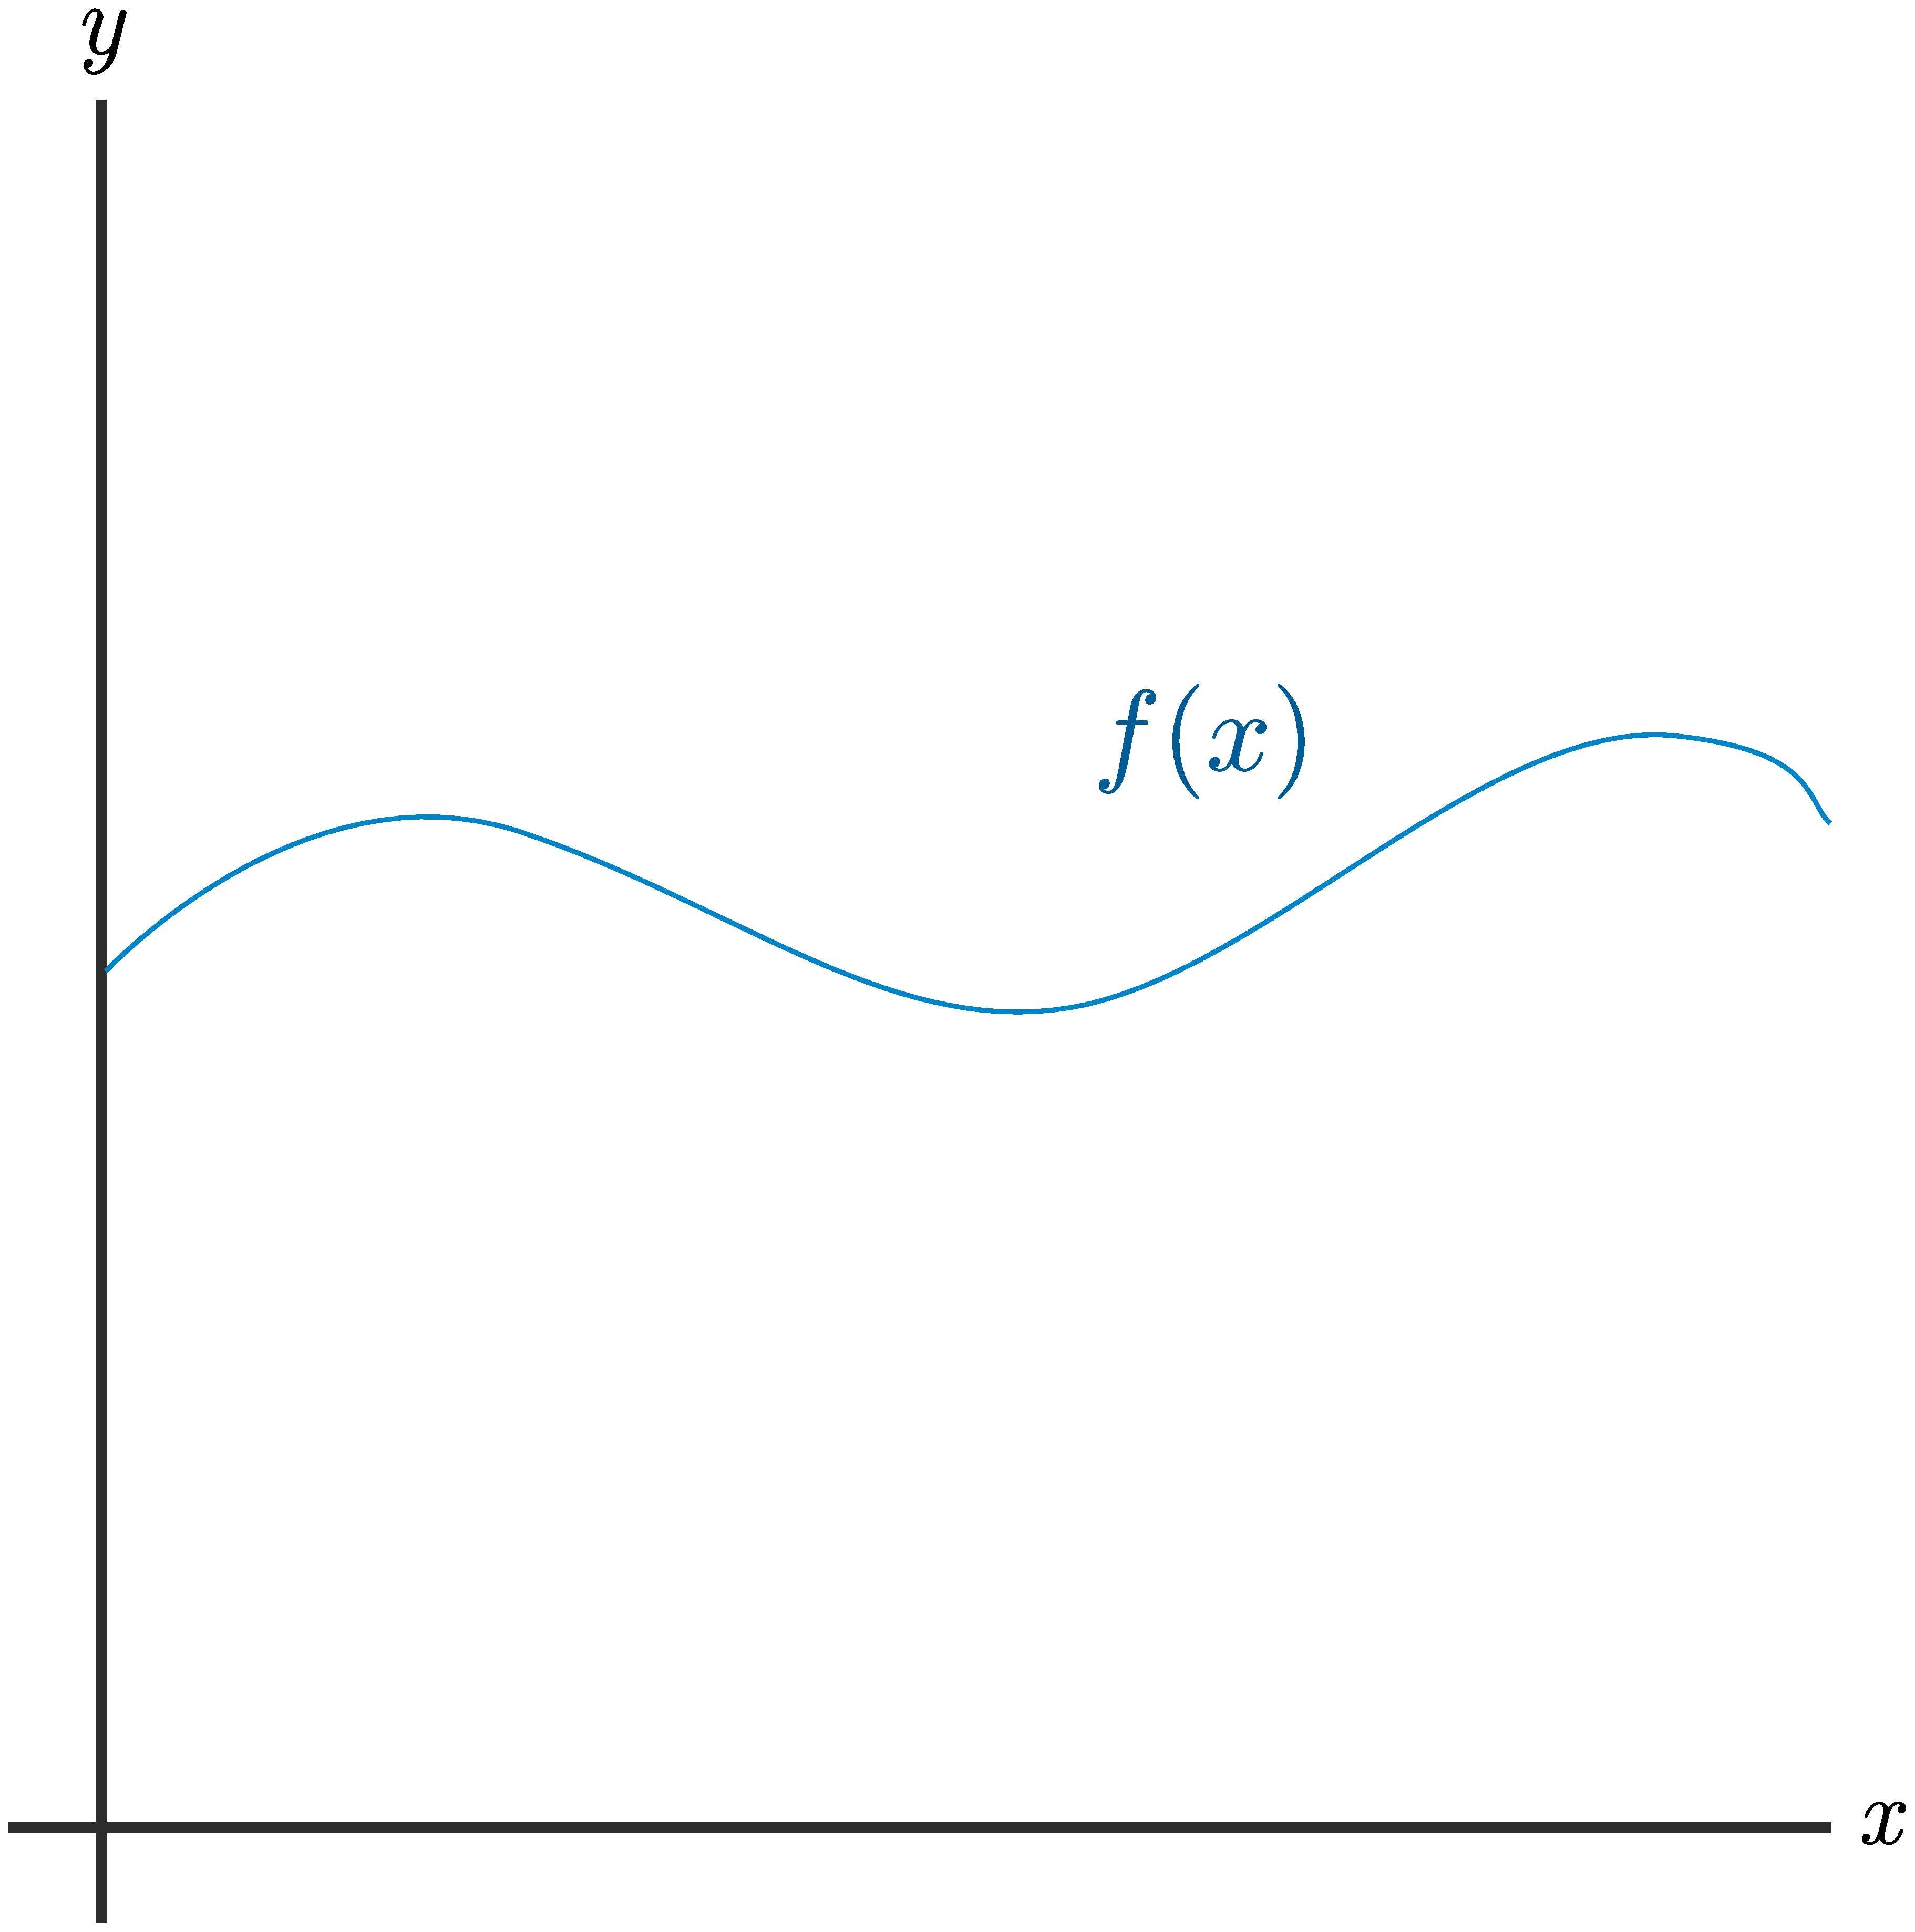
\includegraphics[width=2in]{continuous/integration/rei1.eps}
  \end{center}
  \caption{A curved line.}
  \label{fig:curve}
\end{figure}
\begin{figure}[H]
  \begin{center}
    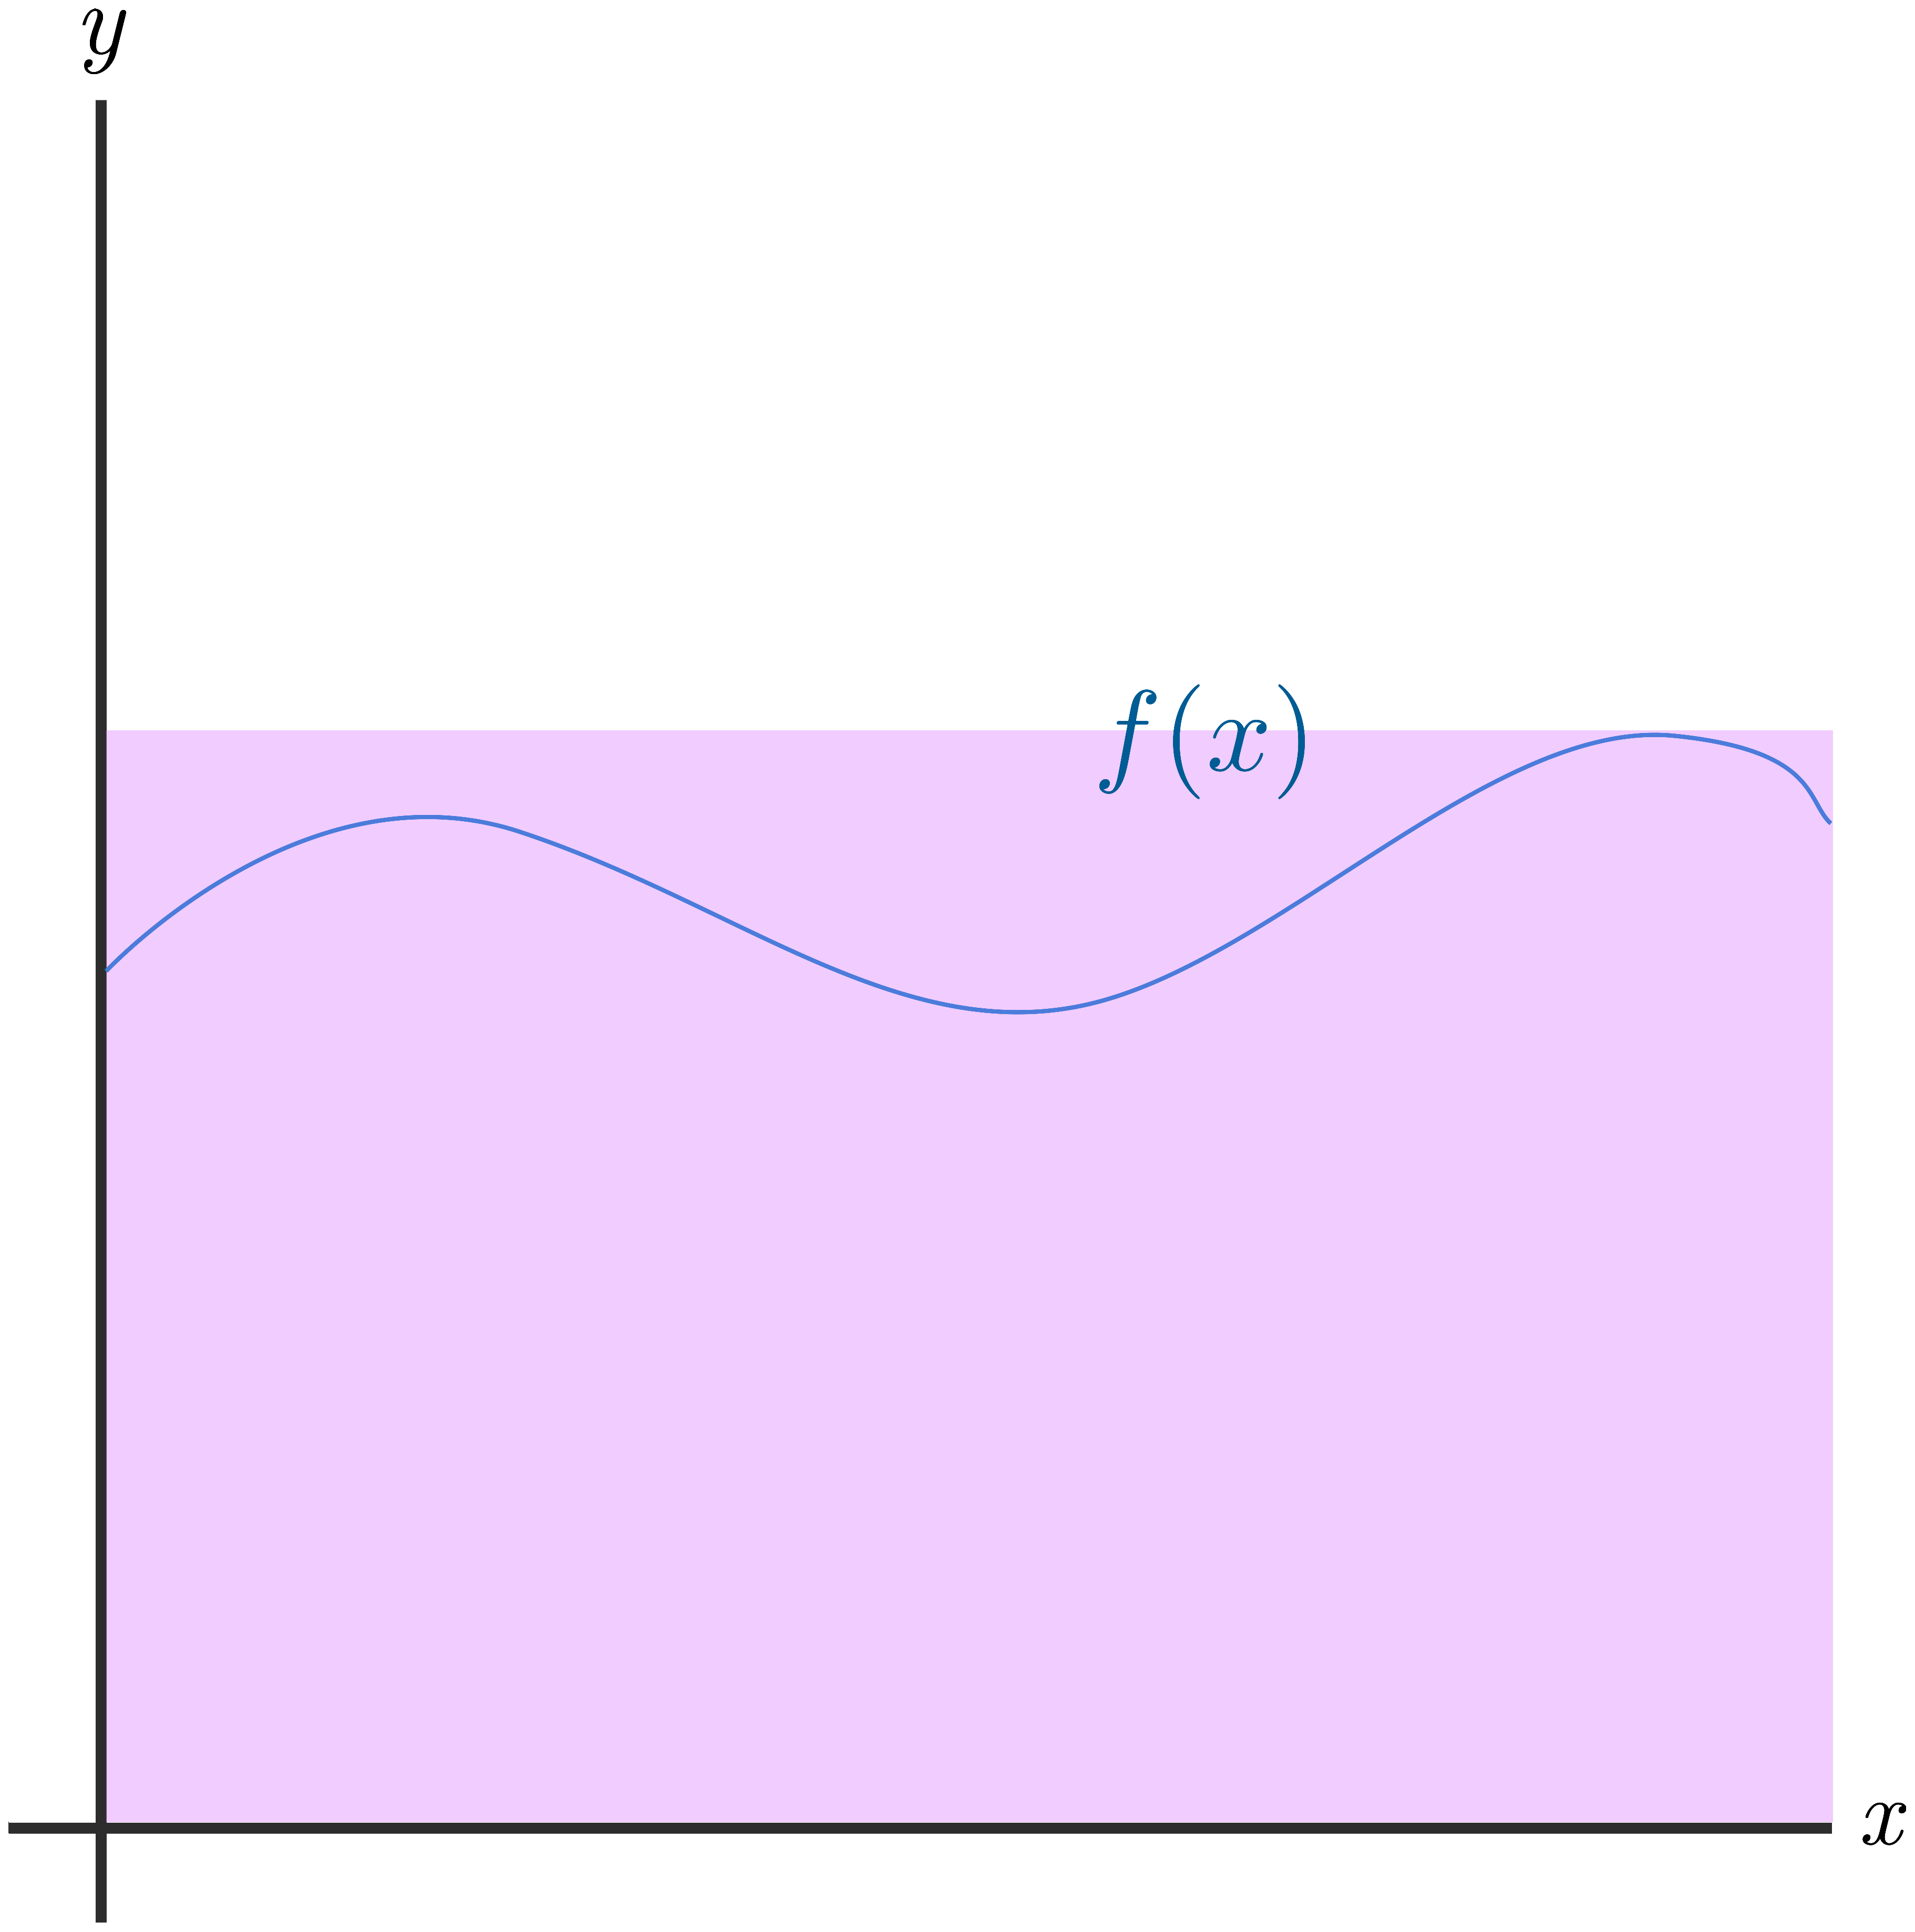
\includegraphics[width=2in]{continuous/integration/rei2.eps}
  \end{center}
  \caption{Approximating the area under the curve with one box.}
\end{figure}
A better estimate would use two boxes.
\begin{figure}[H]
  \begin{center}
    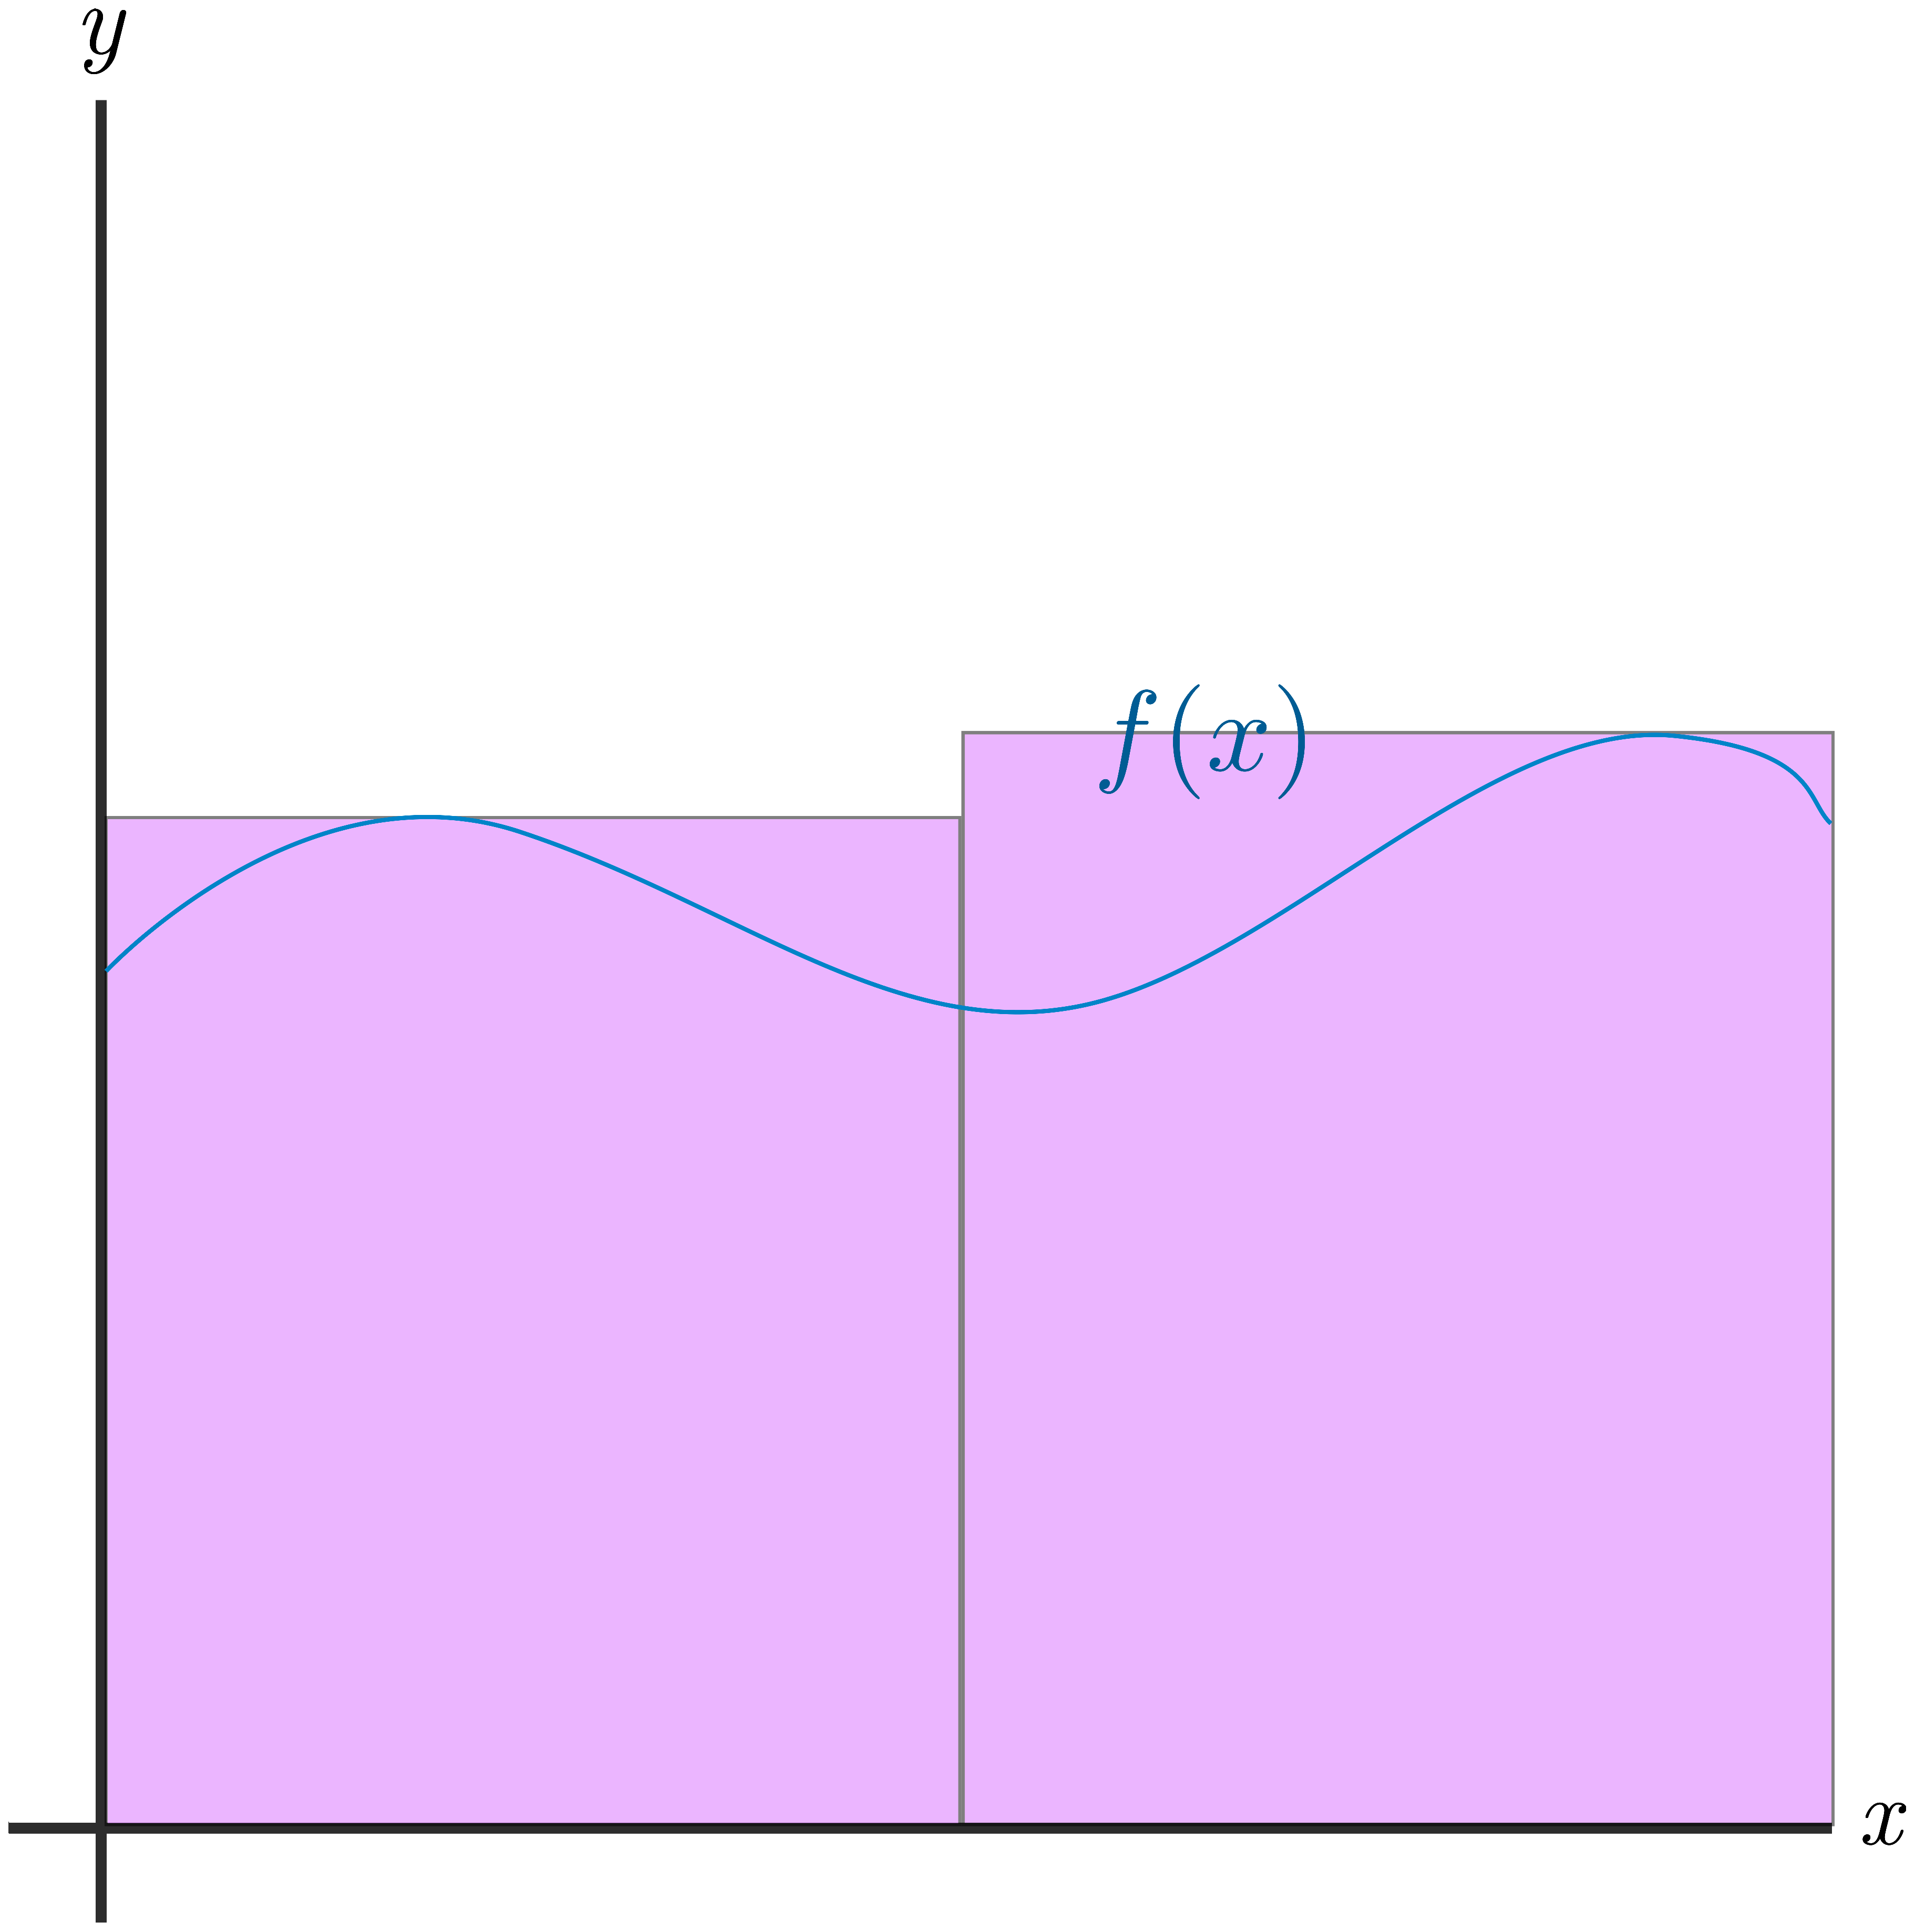
\includegraphics[width=2in]{continuous/integration/rei3.eps}
  \end{center}
  \caption{Approximating the area under the curve with two boxes.}
\end{figure}
Then we could sum the area of both boxes for a closer approximation.
Use more boxes for more and more accurate approximations of the area under the curve.
\begin{figure}[H]
  \begin{center}
    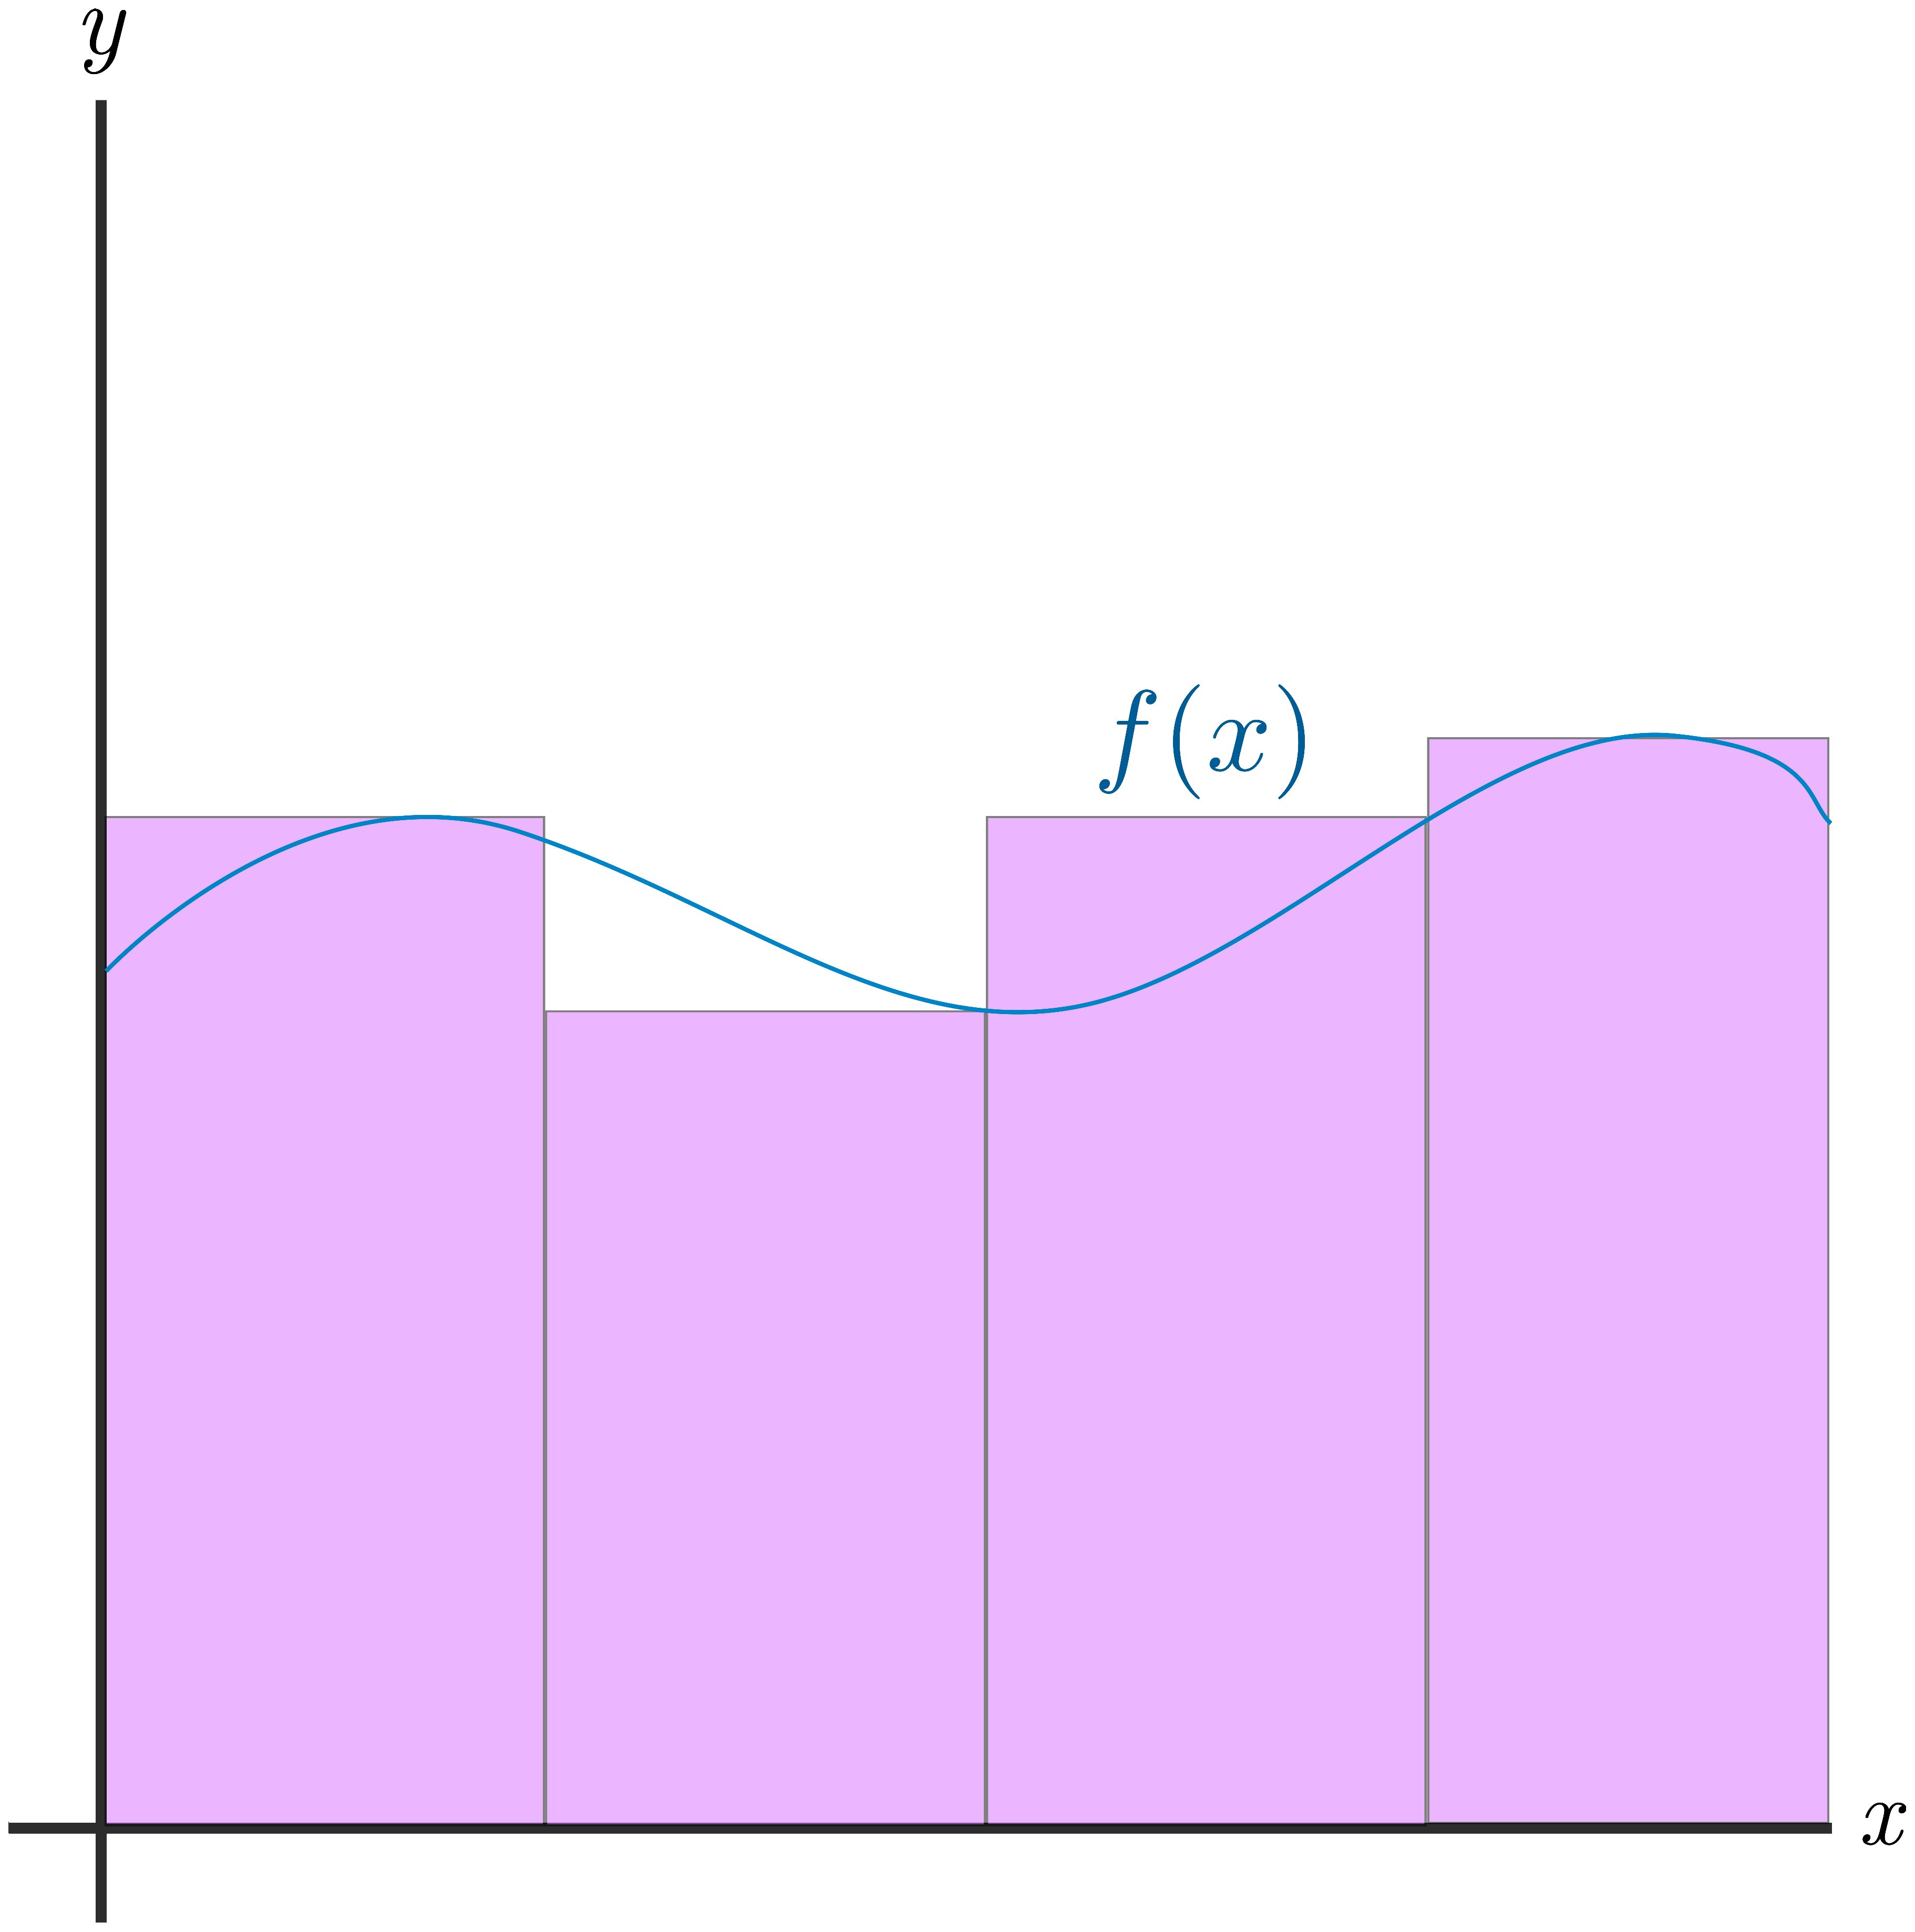
\includegraphics[width=2in]{continuous/integration/rei4.eps}
  \end{center}
\end{figure}
So, if we want to actually calculate something like this, it's handy to define a value $\Delta x$
and let this represent the width of your boxes.
This way we are just measuring different heights, and our width is always constant.
\begin{figure}[H]
  \begin{center}
    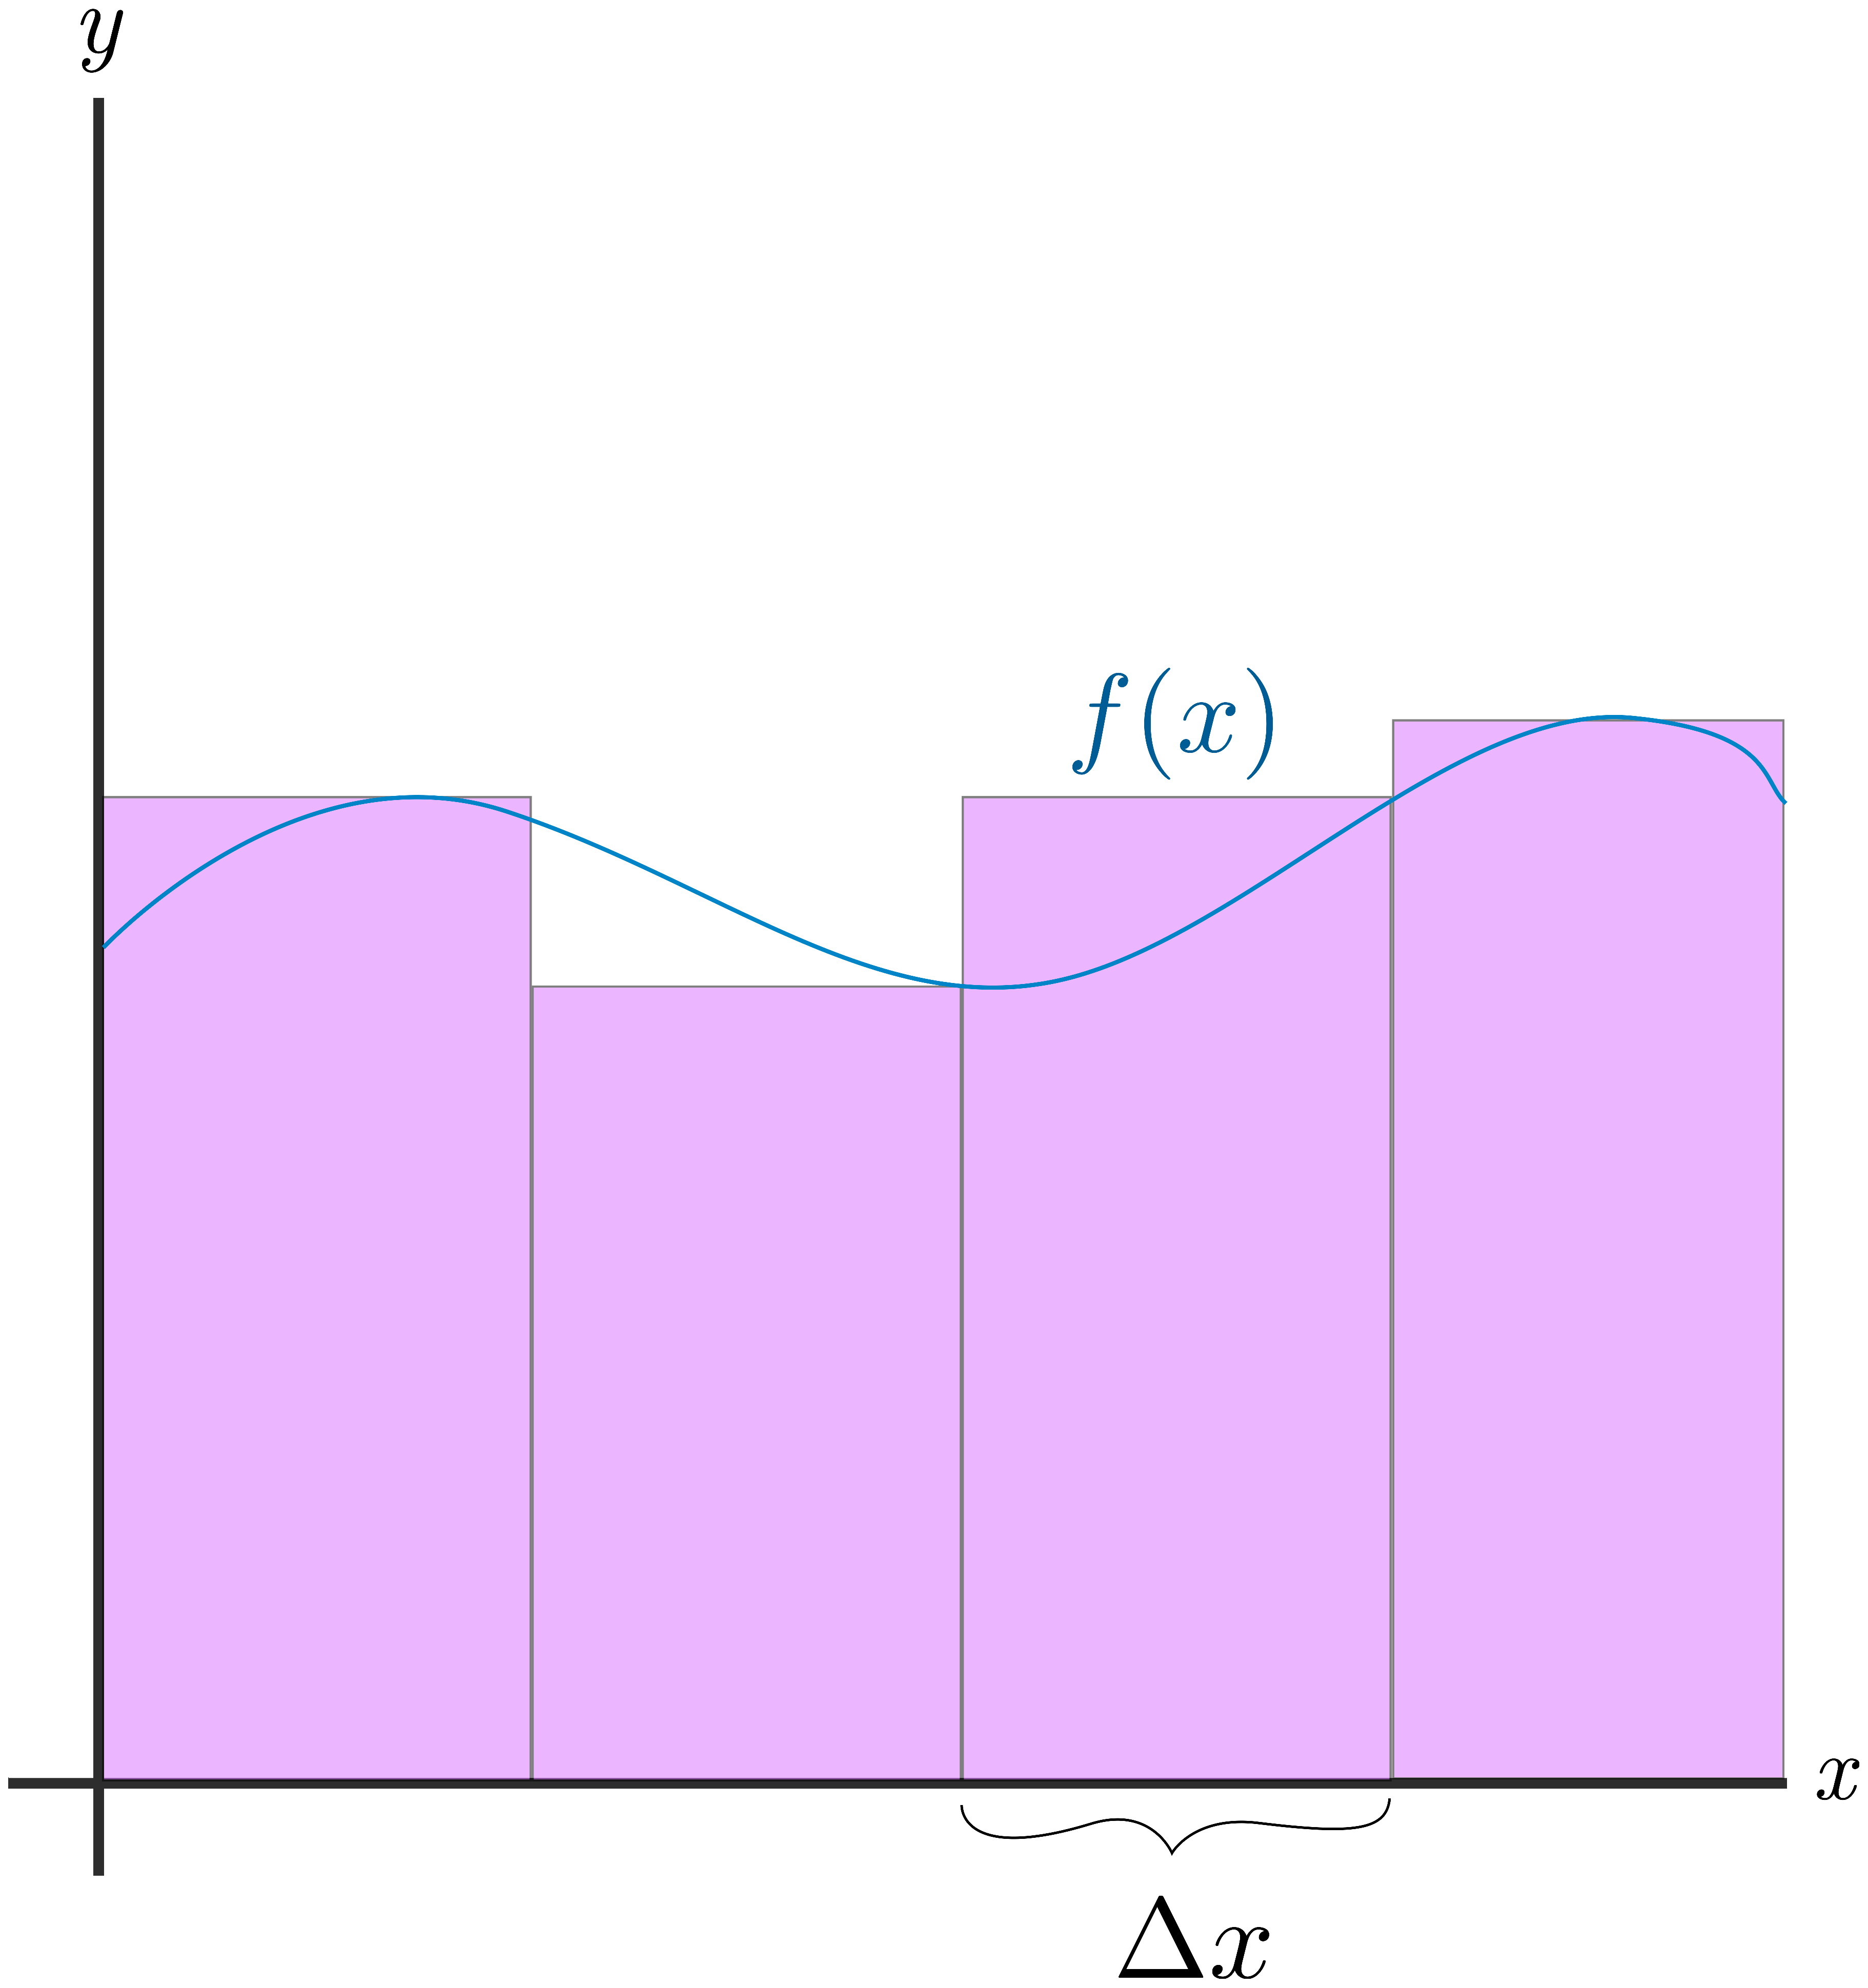
\includegraphics[width=2in]{continuous/integration/rei5.eps}
  \end{center}
  \caption{Approximating the area under the curve with two boxes.}
\end{figure}

\section{Fundamental Theorem of Calculus}
\index{fundamental theorem of calculus}
\begin{theorem}[Fundamental Theorem of Calculus, part 1]
  If $f$ is continuous on $[a,b]$, then $F(x)=\int^x_a f(t)dt$ is continuous on $[a,b]$ and
  differentiable on $(a,b)$ and its derivative is $f(x)$:
  \begin{equation}
    F'(x) = \ddx \int^x_a f(t)\ud t=f(x)
    \label{eq:ftc1}
  \end{equation}
  \cite[p. 276]{thomas}
  \label{th:ftc1}
\end{theorem}
\begin{theorem}
  If $f$ is continuous at every point in $[a,b]$ and $F$ is any antiderivative of $f$ on $[a,b]$, then
  \begin{equation}
    \int^a_b f(x)\ud x=F(b)-F(a).
    \label{eq:ftc2}
  \end{equation}
  \cite[p. 277]{thomas}
  \label{th:ftc2}
\end{theorem}

\section{Basic Integration Formulas}
\label{sec:basicints}
The following are our basic integrals.
We can use this table for reference from time to time,
but as we develop our integration skills, we will become increasingly proficient at using them on-the-spot.

Some are more important than others. For a more complete understanding of these rules, refer to a calculus textbook.
\begin{equation}
  \int k\,\ud x=kx+C \qquad \text{(any number \emph{k})}
\end{equation}
\begin{equation}
  \int x^n \, \ud x = \frac {x^{n+1}}{n+1}+C\,(n \neq -1)
\end{equation}
\begin{equation}
  \int \frac{\ud x}{x}=\ln{|x|}+C
\end{equation}
\begin{equation}
  \int e^x\, \ud x=e^x+C
\end{equation}
\begin{equation}
  \int a^x\, \ud x=\frac{a^x}{\ln a}+C \,(a>0,a\neq 1)
\end{equation}
\begin{equation}
  \int \sin x \, \ud x=-\cos x +C
\end{equation}
\begin{equation}
  \int \cos x \ud x=sin\,x+C
\end{equation}
\begin{equation}
  \int \sec^2x \ud x = \tan x + C
\end{equation}
\begin{equation}
  \int \csc^2 x \ud x = -cot\,x +C
\end{equation}
\begin{equation}
  \int \sec x \tan x \ud x = \sec x +C
\end{equation}
\begin{equation}
  \int \csc x \cot x \,dx = -\csc x +C
\end{equation}
\begin{equation}
  \int \cot x \ud x=\ln{|\sin x|}+C
\end{equation}
\begin{equation}
  \int \cosh x \ud x=\sinh x\,+C
\end{equation}
\begin{equation}
  \int \frac{\ud x}{a^2+x^2}=\frac{1}{a}\arctan{\frac{x}{a}}+C
\end{equation}
\begin{equation}
  \int \frac{\ud x}{\sqrt{a^2+x^2}}=\arcsin{\frac{x}{a}+C} \qquad (a > 0)
\end{equation}

% SECTION COPIED FROM TEXTBOOK
% \section{Integration by Parts}\index{integration by parts}
% % rewrite this.
% Integration by parts is used for simplifying integrals of the form
% \[ \int f(x)g(x) \ud x \text{.} \]
% It is useful when \(f\) can be differentiated repeatedly and $g$ can be integrated repeatedly without difficulty. The integrals
% \[ \int x \cos x \ud x \quad \text{and} \quad \int x^2 e^x \ud x \]
% are such integrals because $f(x)=x$ or $f(x)=x^2$ can be differentiated repeatedly to become zero, and $g(x)=\cos x$ or $g(x)=e^x$ can be integrated repeatedly without difficulty. Integration by parts also applies to integrals like
% \[ \int \ln x \ud x \quad \text{and} \quad \int e^x \cos x \ud x \]
% In the first case, $f(x)=\ln x$ is easy to differentiate and $g(x)=1$ easily integrates to $x$. In the second case, each part of the integrand appears again after repeated differentiation or integration.
%
\section{Integration by Substitution}
Integration by substitution is our simplest technique for evaluating integrals that don't seem to fit into one of our basic rules.
To do these, we must have a grasp on usage of the fundamental integrals from Section \ref{sec:basicints}.
Let's look at an example.
\begin{ex}
  Integrate
  \[
    \int 2e^{2x} \ud x
    \]
  Initially, we don't know how to solve this.
  We know that $\int e^x \ud x$ is just $e^x +C$, but the constant multiplier in the exponent throws us off.
  Notice, however, that the derivative of $2x$, the offending element, is clearly present in the problem: it is $2$.
  This allows us to use a handy trick to make the integrand resemble one that we know how to evaluate.

  Simply let $u=2x$.
  Note that if we perform this subsitution, we would get half the equation in terms of $u$ and the other half in terms of $x$.
  We obviously don't know how to handle this, so we take the derivative of $u$, giving us $\ud u=2$.

  Now we may make our substitutions.
  \begin{align*}
    \int 2e^{2x} \ud x &= \int e^u \ud u \\
    &= e^u +C
    \intertext{ Now we just write this in terms of our original variables.}
    &= e^{2x}+C
  \end{align*}
  And we're done.
\end{ex}

The concept of $u$-substitution isn't tricky.
We should know how to perform substitutions at this point.
What's hard, and what we'll need to practice, is which values to select for our $u$ and $\ud u$.
Remember: look for a piece of the integrand whose derivative is also present in the integrand, and just give it a shot.

If your first substitution fails, don't be discouraged--just try again.

Oftentimes, we won't be lucky enough to see the \emph{exact} derivative in our integrand.
If we're lucky, however, we can usually get within a constant of it, and then we can tweak the integrand to suit our needs.
Let's see what this means.
\begin{ex}
  Integrate.
  \[ \int x (x^2+3/2)^9 \ud x \]
  \begin{sol}
    We can try $u=x^2$, $\ud u=2x$. Unfortunately, we still don't know how to evaluate $(u+3/2)^9$ if we do that.
    It was a good guess, though, and got us closer to an answer. But, wait--$3/2$ is a constant, and should come out when we take its derivative.

    Try letting $u=x^2+3/2$ and $\ud u = 2x \ud x$ instead. This gets us \emph{really} close, except there's no $2$ in our integrand.

    From here, there are two ways to fix this. One is to simply make the righthand side of $\ud u = 2x \ud x$ look how we want it.
    To do this, we simply divide both sides by two.
    This gives us
    \[u=x^2+3/2 \, \frac{\ud u}{2}=x \ud x\]
    Now we're getting somewhere. We can substitute this into our original integral:
    \begin{align*}
      \int x (x^2+3/2)^9 \ud x &= \int u^9 \frac{\ud u}{2} \\
      \intertext{Constants can come out, so this is equal to}
      &= \frac{1}{2} \int u^9 \ud u \\
      \intertext{Awesome! We can integrate this now.}
      &= \frac{1}{2} \frac{u^{10}}{10}+C
      \intertext{Finally, we just replace the $u$ terms with their equivalents in terms of $x$.}
      &= \frac{x^2+3/2}{20}+C
    \end{align*}
    Which is our final answer.
  \end{sol}
\end{ex}
\begin{ex}
  Integrate
  \[ \int (1-x)^{9}\ud x. \]
  \begin{sol}
    Let $u=1-x$ and $\ud u = -\ud x$.
    \begin{align*}
      \int (1-x)^9 \ud x &= -\int u ^9 \\
      &= -\frac{u^{10}}{10}+C\\
      &= -\frac{(1-x)^{10}}{10}+C
    \end{align*}
  \end{sol}
\end{ex}

\section{Integration By Parts Formula}
\index{integration by parts}

Integration by parts is a method of separating out elements of integrals that we don't know how to evaluate, and taking their derivative instead.

Its formula comes from our definition for the derivative product rule:
  \begin{align*}
    \frac{\ud}{\ud x}\big[ f(x) g(x) \big] &= f'(x)g(x)+f(x)g'(x) \\
    \intertext{If we take the indefinite integral of each side,}
    \int \frac{\ud}{\ud x}\big[ f(x) g(x) \big] \ud x &= \int \big[f'(x)g(x)+f(x)g'(x)\big] \ud x\\
    \intertext{Now separate out the terms in the righthand side.}
    \int \frac{\ud}{\ud x}\big[ f(x) g(x) \big] \ud x &= \int f'(x)g(x)\ud x +\int f(x)g'(x) \ud x \\
    \intertext{From here, we note that the integral and deriviative in the lefthand side cancel each other out, if we use the fundamental theorem of calculus.}
    f(x)g(x) &= \int f'(x)g(x)\ud x +\int f(x)g'(x) \ud x \\
    \intertext{Now, subtract the first integral from both sides.}
    f(x)g(x) -\int f'(x)g(x) \ud x &= \int f(x)g'(x) \ud x \\
    \intertext{Swap the left and righthand sides, and we have the formula for integration by parts!}
     \int f(x)g'(x) \ud x&=f(x)g(x) -\int f'(x)g(x) \ud x \\
  \end{align*}
  For convenience, we can rewrite this formula in terms of $u$, $\ud u$, $\ud v$, and $v$ as follows:
\begin{equation}
  \int u \ud v =  uv - \int v \ud u
  \label{equation:intbyparts}
\end{equation}
The real goal, here, is to always make $\int v \ud u$ easier to evaluate than $\int u \ud v$.
It doesn't really matter what $u$ and $v$ are.
Learning when to use integration by parts can be tricky, and learning which parts are best assigned where is even more difficult.
Generally, this takes a fair amount of examples, coupled with considerable practice for one to develop an efficient intuitive understanding.
\begin{ex}
  Integrate
  \[
    \int x \cos x \ud x.
    \]
    \begin{sol}
      We use integration by parts with
      \begin{align*}
        u&= x & \ud v &= \cos x \\
        \ud u &= \ud x & v &= \sin x
      \end{align*}
      So our integral becomes something we can integrate.
      \begin{align*}
        \int x \cos x \ud x &= x \sin x - \int \sin x \ud x \\
        &= x \sin x + \cos x +C
      \end{align*}
    \end{sol}
\end{ex}
A note on selecting $u$ and $\ud v$: it is usually easiest to pick $\ud v$ first to be everything we know how to integrate, including the $\ud x$, and then let $u$ be the rest.
This is just a guideline, however, and one we will frequently have to bend.
\begin{ex} A tough integration by parts problem.\footnote{Solved by Dr. James Martin, CNU Department of Mathematics. \url{http://math.cnu.edu/martin.htm}}
	\[ \int \frac{xe^{2x}}{(2x+1)^2}\ud x \]
  \begin{sol}
      We use integration by parts as follows:
      \begin{align*}
        u&=e^{2x} & \ud v&=\frac{x}{(2x+1)^2} \\
        \ud u &= 2e^{2x} & v &=\frac{1}{4+8x}+\frac{\ln{(1+2x)}}{4}
      \end{align*}
      To get:
      \begin{align*}
        \int \frac{xe^{2x}}{(2x+1)^2}\ud x
        =& \frac{e^{2x}}{4+8x}+\frac{e^{2x}\ln{|1+2x|}}{4}-\int 2e^{2x}\left[\frac{1}{4+8x}+\frac{\ln{(1+2x)}}{4}\right]\ud x \\
      \end{align*}
      Then we simplify the integrand.
      \begin{align*}
        \int \frac{xe^{2x}}{(2x+1)^2}\ud x =& \frac{e^{2x}}{4+8x}+\frac{e^{2x}\ln{|1+2x|}}{4}-\int \frac{2e^{2x}}{4+8x}\ud x-\frac{1}{2} \int e^{2x}\ln{|1+2x|}\ud x \\
        =& \frac{e^{2x}}{4+8x}+\frac{e^{2x}\ln{|1+2x|}}{4}-\frac{1}{2}\int \frac{e^{2x}}{1+2x}\ud x-\frac{1}{2} \int e^{2x}\ln{|1+2x|}\ud x
      \end{align*}
      We use integration by parts again on the second integral as follows:
      \begin{align*}
        u=&\ln{|1+2x|} & \ud v=&e^{2x} \\
        \ud u=&\frac{2}{1+2x}\ud x & v=& \frac{1}{2}e^{2x}
      \end{align*}
      \begin{align*}
        =& \frac{e^{2x}}{4+8x}+\frac{e^{2x}\ln{|1+2x|}}{4}
        -\frac{1}{2}\left[\frac{1}{2}e^{2x}\ln{|1+2x|}
          -\frac{1}{2} \int \frac{2e^{2x}}{1+2x} \ud x\right]
          -\frac{1}{2}\int \frac{e^{2x}}{1+2x}\ud x \\
          \intertext{We simplify our result, and all but one of the terms cancel:}
          =& \frac{e^{2x}}{4+8x}+\frac{e^{2x}\ln{|1+2x|}}{4}
          -\frac{1}{4}e^{2x}\ln{|1+2x|}
          + \frac{1}{2} \int \frac{e^{2x}}{1+2x} \ud x
          -\frac{1}{2}\int \frac{e^{2x}}{1+2x}\ud x \\
          =& \frac{e^{2x}}{4+8x}+\frac{e^{2x}\ln{|1+2x|}}{4}
          -\frac{e^{2x}\ln{|1+2x|}}{4}+C \\
          =& \frac{e^{2x}}{4+8x}+C
        \end{align*}
\end{sol}
\end{ex}
\begin{ex}
  Integrate
  \[\int\ln x \ud x.\]
  \begin{sol}
  Since $\int \ln x \ud x$ can be written as $\int \ln x \cdot 1 \ud x$, we can use integration by parts as follows:
  \begin{align*}
    u&=\ln x & \ud v &= \ud x \\
    \ud u &= \frac{\ud x }{x} & v&=x
  \end{align*}
  Which gives us the integral
  \begin{align*}
    \int\ln x \ud x &=
      x \ln x - \int  \frac{x \ud x}{x} \\
      &= x \ln x - \int \ud x \\
      &= x \ln x - x + C
    \end{align*}
  \end{sol}
\end{ex}

\subsection{Integration by Parts Cheat Sheet}
This is a set of guidlines\footnote{Proposed by Herbert Kasube of Bradley University.} advising whichever part of an integral comes first in this list should be assigned to $u$.
\begin{enumerate}
  \item Logarithms
  \item Inverse functions
  \item Algebraic
  \item Trigonometric
  \item Exponential
\end{enumerate}


% \subsection{Reduction Formulas}
% % probably rewrite this. I think I might have too much unoriginal material in this section.
% Consider the integral
% \begin{align*}
%   I_n=&\int x^n e^{ax} \ud x
%   \intertext{Integration by parts gives you}
%   I_n=&x^n \frac{1}{a}e^{ax}-\int nx^{n-1}\frac{1}{a}e^{ax}\ud x \\
%      =&\frac{1}{a}x^ne^{ax}-\frac{n}{a}\int x^{n-1}e^{ax}\ud x
% \end{align*}
% We haven't computed the integral. What we have done is derived the following \textbf{reduction formula}
% \begin{equation}
%   I_n=\frac{1}{a}x^ne^{ax}-\frac{n}{a}I_{n-1}
% \end{equation}
% which holds for all $n$.
%
% For $n=0$ the reduction formula says
% $$ I_0=\frac{1}{a}e^{ax} \to \int e^{ax}\ud x = \frac{1}{a}e^{ax}+C $$
%
% When $n \neq 0$ the reduction formula tells us that we have to compute $I_{n-1}$ if we want to find $I_n$. The point of a reduction formula is that the same formula also applies to $I_{n-1}$, and $I_{n-1}$, etc. so that after repeated application of the formula we end up with $I_0$, an integral we know how to compute.\cite{freenotes}
% \begin{ex}
%   %[textbook: \#4/pg.441]
%   Integrate
%   \[ \int e^x \cos x \ud x \]
%   \begin{sol}
%     We use integration by parts with
%     \begin{align*}
%       u &= \cos x & \ud v &= e^x \ud x \\
%       \ud u &= - \sin x \ud x & v &=e^x
%     \end{align*}
%     Which gives us the integral
%     \begin{align*}
%       \int e ^x \cos x \ud x &= e^x \cos x - \int -e^x \sin x \ud x \\
%       &= e^x \cos x+ \int e^x \sin x \ud x \\
%       \intertext{Now we use $u$-substitution with $u=e^x$ and $\ud u = e^x \ud x$.}
%       &= e^x \cos x + \int \sin u \ud u \\
%       &= e^x \cos x - \cos u +C \\
%       &= e^x \cos x - \cos {e^x} +C
%     \end{align*}
%   \end{sol}
% \end{ex}
\begin{ex}
  Integrate:
  \[
    \int 3x^2 \cos x^3 \ud x
    \]
  \begin{sol}
    This is not an integration by parts problem.
    Because we can spot the derivative of $x^3$ clearly in the integrand,
    we can let $u=x^3$ and $\ud u = 3x^2 \ud x$.
    \begin{align*}
      \int 3x^2 \cos x^3 \ud x & = \int \cos u \ud u \\
      &= \sin u +C\\
      &= \sin {x^3}+C
    \end{align*}
  \end{sol}
\end{ex}
\begin{ex}
  Integrate
  \[
    \int x \cos x \ud x
    \]
    \begin{sol}
      Use integration by parts with
      \begin{align*}
        u &= x & \ud v &= \cos x \ud x \\
        \ud u &= \ud x & v &= \sin x
      \end{align*}
      Which gives us
      \begin{align*}
        \int x \cos x \ud x &= x \sin x - \int \sin x \ud x \\
        &= x \sin x + \cos x +C
      \end{align*}
    \end{sol}
\end{ex}
\begin{ex}
  Integrate
  \[
    \int x e^x \ud x
    \]
    \begin{sol}
      Use integration by parts with
      \begin{align*}
        u&=x & \ud v &= e^x \ud x \\
        \ud u &= \ud x & v &= e^x
      \end{align*}
      \begin{align*}
        \int x e^x \ud x &= x e^x -\int e^x \ud x \\
        &=x e^x -e^x +C
      \end{align*}
    \end{sol}
\end{ex}
\begin{ex}
  Integrate
  \[
    \int x \ln x \ud x
    \]
  \begin{sol}
    Use integration by parts with
    \begin{align*}
      u&= \ln x & \ud v &= x \ud x \\
      \ud u &= \frac{\ud x}{x} & v &= \frac{x^2}{2}
    \end{align*}
    Which gives us
    \begin{align*}
      \int x \ln x &= \frac{x^2 \ln x}{2}- \int \frac{x^2 \ud x}{2x} \\
      &= \frac{x^2 \ln x}{2}-\frac{1}{2} \int x \ud x \\
      &= \frac{x^2 \ln x}{2}-\frac{x^2}{4}+C
    \end{align*}
  \end{sol}
\end{ex}
\begin{ex}
  \[
    \int x e^{x^2} \ud x
    \]
    \begin{sol}
      This looks like an integration by parts problem at first, but again it is just a regular $u$-substitution problem.
      Let $u=x^2$ and $\ud u=2x\ud x$.
      \begin{align*}
        \int x e^{x^2} \ud x &= \frac{1}{2}e^u \ud u \\
        &= \frac{1}{2} e^u +C \\
        &= \frac{1}{2}e^{x^2} +C
      \end{align*}
    \end{sol}
\end{ex}
% PLEASE rewrite this section ASAP.
% Clean it up, add descriptions, put it in proper format, etc.
% This is priority #1 for now.
%
%  \begin{ex}
%    \[ \int x^3 e^{x^2} \ud x \]
%    Don't be discouraged if your first attempt at integration by parts fails.
%    \begin{align*}
%      u &= x^{3} & dv &= e^{x^{2}} \\
%      \ud u &= 3x^{2} \ud x & v &= \text{?}
%    \end{align*}
%    Just try again:
%    \begin{align*}
%      u &= x^2 & dv &= x e^{x^2} \ud x \\
%      \ud u &= 2x \ud x & v &= \frac{e^{x^2}}{2}
%    \end{align*}
%    \begin{align*}
%      \int x^3 e^{x^2} \ud x &=
%      \frac{x^2 e^{x^2}}{2} - \int \frac{2}{2} x e^{x^2} \ud x
%      =\frac {x^2 e^x}{2}- \frac {e^{x^2}}{2} + C \\
%      &=\frac{x^2 e^x-e^x}{2}+C
%    \end{align*}
%  \end{ex}
%  \begin{ex}
%    \[ \int e^x (x+1)^2 \ud x \]
%    Start with integration by parts:
%    \begin{align*}
%      u &= (x+1)^2 & \ud v &= e^x \ud x \\
%      \ud u &= 2(x+1)\ud x & v &= e^x
%    \end{align*}
%    \begin{align*}
%      \int e^x (x+1)^2 \ud x&=
%        e^x (x+1)^2 - \int e^x 2(x+1)\ud x \\
%      &=e^x (x+1)^2 - 2\int e^x (x+1)\ud x
%    \end{align*}
%    Saving this for later...
%    \begin{comment}
%    Then use integration by parts again:
%    \begin{align*}
%      u &= x+1 & \ud v &= e^x \ud x \\
%      \ud u &= \ud x & v &= e^x
%    \end{align*}
%    \begin{align*}
%      \int e^x (x+1)^2 \ud x&=
%        e^x (x+1)^2 - 2\left[e^x(x+1)-\int e^x \ud x \right] \\
%      &=e^x (x+1)^2 - 2[e^x(x+1)-e^x] + C \\
%      &=e^x (x+1)^2 - 2e^x(x+1)+2e^x + C\\
%      &=x^2e^x+e^x-2xe^x-2e^x+2e^x+C
%    \end{align*}
%    \end{comment}
%  \end{ex}
%  \begin{ex}
%    Another ``strange'' integral:
%    \[ \int \arcsin x \ud x \]
%  \end{ex}
%  \begin{ex}
%    \[ \int \sin^{-1}x \ud x \]
%    \begin{align*}
%      u &= \sin^{-1}x & \ud v&=\ud x\\
%      \ud u &= \frac {1}{\sqrt{1-x^2}} \ud x & v &= x
%    \end{align*}
%    \begin{align*}
%      \int \sin^{-1}x \ud x &=
%      x \sin^{-1}x - \underbrace{\int \frac {x}{\sqrt{1-x^{2}}} \ud x}_{\lets u = 1-x^{2}}=x \sin^{-1}x-\frac{1}{2} \int \frac{\ud u}{\sqrt{u}} \\
%      &=x \sin^{-1}x+\frac{1}{2} \int u^{-1/2}\ud u=x sin^{-1}x+\sqrt u +C \\
%      &=x \sin^{-1}x+\sqrt{1-x^{2}} +C
%    \end{align*}
%  \end{ex}
%  \begin{ex}
%    \[ \int 4x e^{4x} \ud x \]
%    \begin{sol}
%    We use integration by parts with
%    \begin{align*}
%      u&=x & \ud v&=e^{4x}\ud x \\
%      \ud u &=\ud x & v &=\frac{1}{4}e^{4x}
%  	\end{align*}
%  	\begin{align*}
%  	  \frac{1}{x^4+2x^2+1}
%  	    =&4\left[x \cdot \frac{1}{4}e^{4x}-\int 1 \cdot \frac{1}{4} e^{4x} \ud x\right] \\
%  	    =&4\left[x \cdot \frac{1}{4}e^{4x}-\frac{1}{4}\int e^{4x} \ud x\right] \\
%  	    =& x e^{4x}-\frac{1}{4}e^{4x} + C
%    \end{align*}
%  \end{sol}
%  \end{ex}
%
%  % \begin{homework}
%  % pg. 489 odd 1-7, pg. 441 odd 1-23, pg. 441 6, 8, 35, 39.
%  % \end{homework}
%
%  \begin{ex}[\#23/pg.441]
%    \[ \int e^{2x}\cos{3x}\ud x \]
%    \begin{align*}
%      u &= \cos{3x} & \ud v&=e^{2x}\ud x\\
%      \ud u &= -3\sin{3x}\ud x & v&=\frac{1}{2}e^{2x}
%    \end{align*}
%    \begin{align*}
%      \int e^{2x}\cos{3x}\ud x &=
%        \frac{1}{2}e^{2x}\cos{3x}+\frac{3}{2}\int e^{2x}\sin{3x}\ud x \\
%      &=\frac{1}{2}e^{2x}\cos{3x}+\frac{3}{2}
%        \left[\frac{1}{2}e^{2x}\sin{3x}-\frac{3}{2}\int e^{2x}\cos{3x}\ud x \right]\ \\
%      \to\frac{4}{4}\int e^{2x}\cos{3x}\ud x
%        &=\frac{1}{2}e^{2x}\cos{3x}+\frac{3}{4}e^{2x}\sin{3x}-\frac{9}{4}\int e^{2x}\cos{3x}\ud x \\
%      \frac{13}{4}\int e^{2x}\cos{3x}\ud x
%        &=\frac{1}{2}e^{2x}\cos{3x}+\frac{3}{4}e^{2x}\sin{3x}+C \\
%      13\int e^{2x}\cos{3x}\ud x
%        &=2e^{2x}\cos{3x}+3e^{2x}\sin{3x}+C \\
%      \int e^{2x}\cos{3x}\ud x
%        &=\frac{2}{13}e^{2x}\cos{3x}+\frac{3}{13}e^{2x}\sin{3x}+C \\
%      &=\frac{e^{2x}}{13}\left[2\cos{3x}+3\sin{3x}\right]+C
%    \end{align*}
%    % Old in-class garbage:
%    % $$\frac{1}{2}cos(3x)e^{2x}+\frac{3}{2}\int e^{2x}sin(3x)\ud x \frac{1}{2}cos(3x)e^{2x}+\frac{3/2} (\frac{1}{2}e^{2x}sin(3x)-\frac{3}{2}\int e^{2x}cos(3x)\ud x)
%  \end{ex}
%  \begin{ex}
%    Integrate
%    \[ \int x^2\cos{3x}\ud x \]
%    \begin{sol}
%      Use integration by parts.
%      \begin{align*}
%        u&=x^2 && \ud v=\cos{3x}\ud x \\
%        \ud u=&2x\ud x && v=\frac{1}{3}\sin{3x}
%      \end{align*}
%      \begin{align*}
%        \int x^2\cos{3x}\ud x
%        =nt^{a}_{-\infty} f(x) \ud x
%            + \int^{\infty}_{a} f(x) \ud x& \frac{1}{3}x^2\sin{3x}-\frac{2}{3}\int x \sin{3x} \ud x \\
%        \intertext{Now use integration by parts again}
%        =& \frac{1}{3}x^2\sin{3x}-\frac{2}{3} \left( \frac{-x}{3}\cos{3x}+\frac{1}{3}\int\cos{3x}\ud x \right)\\
%        =& \frac{1}{3}x^2\sin{3x}+\frac{2}{9}x\cos{3x}-\frac{2}{27}\sin{3x}+C
%      \end{align*}
%    \end{sol}
%  \end{ex}
%  \begin{ex}
%    Integrate
%    \[ \int \frac{x}{\sqrt{x+3}} \]
%    \begin{sol}
%    Use integration by parts with
%    \begin{align*}
%      u&=x  & \ud v&=\frac{\ud x}{\sqrt{x+3}} \\
%      \ud u&=\ud x & v &=2\sqrt{x+3}
%    \end{align*}
%    \begin{align*}
%      \int \frac{x}{\sqrt{x+3}} =& 2x\sqrt{x+3}-\int 2\sqrt{x+3}\ud x \\
%      =& 2x \sqrt{x+3}-\frac{4}{3}(x+3)^{3/2}+C
%    \end{align*}
%  \end{sol}
%  \end{ex}
%  \begin{ex}
%    Integrate
%    \[\sin^{-1}{3x}\ud x\]
%    \begin{sol}
%      We use integration by parts with
%      \begin{align*}
%        u&=\arcsin{3x} & \ud v &= \ud x \\
%        \ud u &=\frac{3}{\sqrt{1-9x^2}}\ud x & v&=x
%      \end{align*}
%      \begin{align*}
%        \arcsin{3x}\ud x
%        =&x\arcsin{3x}-\int \frac{3x \ud x}{\sqrt{1-9x^2}} \\
%        =&x\arcsin{3x}+\frac{1}{3}\sqrt{1-9x^2}+C
%      \end{align*}
%    \end{sol}
%  \end{ex}


\section{Trigonometric Integrals}

To solve trigonometric integrals (that is, integrals already involving trigonometric functions),
we often have to do a fair amount of playing around with trigonometric identities in order to make them possible.
A technique we can use to further this is separating out trigonometric operators that are in powers, such that we may perform substitution on them.

Take the following integral, for example.
\begin{ex}
  Integrate.
  \[\int \cot^2x \csc^4x \ud x \]
  \begin{sol}
    Separate a $\csc^2x$ from the integrand.
    \begin{align*}
      \int \cot^2x \csc^4x \ud x
      =& \cot^2x \csc^2x \csc^2x \ud x
    \end{align*}
    Remembering our basic trig identity
    \[ \sin^2x + \cos^2x = 1\]
    we can divide through by $\sin^2x$ to get
    \[ 1+\cot^2x=\csc^2x \]
    and substitute that into our new integral
    \begin{align*}
      \int\cot^2x\csc^2x\csc^2x\ud x
      =& \int \cot^2x (1+\cot^2x)\csc^2x \ud x \\
      \intertext{Now we let $u=\cot x$ and $\ud u=\csc^2x \ud x$.}
      =&\int u^2(1+u^2)\ud u \\
      \intertext{which we can do.}
      =& \frac{u^3}{3}+\frac{u^5}{5}+C \\
      \intertext{Now replace our old $u$-substitutions}
      =& \frac{\cot^3x}{3}+\frac{\cot^5x}{5}+C
    \end{align*}
  \end{sol}
\end{ex}


% Trigonometric integrals involve algebraic combinations of the six basic trigonometric functions. In principle, we can always express such integrals in terms of sines and cosines, but it is often simpler to work with other functions, as in the integral
% $$ \int sec^2 x \ud x = \tan x + C $$
% The general idea is to use identities to transform the integrals we have to find into integrals that are easier to work with.
%
% We begin with integrals of the form:
% $$ \int \sin^mx\cos^nx\ud x $$
% where $m$ and $n$ are nonnegative integers (positive or zero). We can divide the appropriate substitution into three cases according to $m$ and $n$ being odd or even.
% \begin{enumerate}
%   \item If \textbf{$m$ is odd}, we write $m$ as $2k+1$ and use the identity $\sin^2x=1-\cos^2x$ to obtain
%   $$sin^mx=sin^{2k+1}x=(sin^2x)^k\sin x=(1-\cos^2x)^k\sin x $$
%   Then we combine the single $\sin x$ with $\ud x$ in the integral and set $\sin x \ud x$ equal to $-\ud (\cos x)$.
%   \item If \textbf{$m$ is even and $n$ is odd} in $\int \sin^mx\cos^nx \ud x$, we write $n$ as $2k+1$ and use the identity $\cos^2x=1-\sin^2x$ to obtain
%   $$ \cos^nx=\cos^{2k+1}x=(\cos^2x)^k\cos x=(1-\sin^2x)^k\cos x $$
%   We then combine the single $\cos x$ with $\ud x$ and set $\cos x \ud x$ equal to $d(\sin x)$.
%   \item If \textbf{both $m$ and $n$ are even} in $\int \sin^mx\cos^nx\ud x$, we subsitute
%   \begin{align*}
%     &\sin^2x=\frac{1-\cos{2x}}{2}
%     &\cos^2x=\frac{1+\cos{2x}}{2}
%   \end{align*}
%   to reduce the integrand to one in lower powers of $\cos{2x}$.
% \end{enumerate}

We can also use trigonometric identities to eliminate square roots in integrals:
\begin{ex}
  \[ \int^{\frac{\pi}{4}}_{0} \sqrt{1+\cos{4x}}\ud x \]
  To eliminate the square root, we use the identity
  \[ \cos^2 \theta = \frac{1+\cos{2 \theta}}{2} \]
  With $\theta=2x$, this becomes:
  \[ 1+\cos{4x}=2\cos^2{2x} \]
  Therefore,
  \begin{align*}
    \int^{\frac{\pi}{4}}_{0} \sqrt{1+\cos{4x}}\ud x&= \int^{\frac{\pi}{4}}_{0} \sqrt{2 \cos^2{2x}} \ud x = \int^{\frac{\pi}{4}}_{0} \sqrt2 \sqrt{\cos^2{2x}} \\
    &= \sqrt2 \int^{\frac{\pi}{4}}_{0} |\cos{2x}|\ud x = \sqrt2 \int^{\frac{\pi}{4}}_{0} \cos{2x}\ud x \\
    &= \sqrt2 \left[\frac{\sin{2x}}{2}\right]^{\frac{\pi}{4}}_{0} = \frac{\sqrt2}{2}[1-0] \\
    &= \frac{\sqrt2}{2}
  \end{align*}
\end{ex}
\begin{comment}
  I don't like how this is structured.
  \begin{itemize}
      \item $ \int tan^{\text{power}}x \, sec^{\text{even}}x\ud x$
      \item $ \int \underbrace{sin^{\text{power}x} \, cos^{\text{power}}x \ud x}_{\text{except where both are even}} $
      \item $ \int cot^{\text{power}x} \, csc^{\text{even}}x \ud x $
      \item $ \int sin(mx) \,  sin(nx) \ud x = \int \frac{1}{2}(cos(m-n)x-cos(m+n)x)$
      \item $ \int cos(mx) \,  cos(nx) \ud x = \int \frac{1}{2}(cos(m-n)x-cos(m+n)x)$
  \end{itemize}
\end{comment}

\begin{ex}
  \[ \int \sin^7x \cos^2x \ud x \]
  \begin{sol}
  \begin{align*}
    \int \sin^7x \cos^2x \ud x &=
      \int \sin^6x \cos^2x \sin x \ud x \\
    &=(\sin^2x)^3\cos^2x\sin x\ud x \\
    \intertext{because $\sin^2x=1-\cos^2x$}
    &=(1-\cos^2x)^3 \cos^2x\sin x \ud x
    \intertext{let $u=\cos x$ and $\ud u=-\sin x$.}
    &=-\int(1-u^2)^3u^2\ud u \\
    &=-\int (1-u^2)(1-u^2)(1-u^2)u^2\ud u \\
    &=-\int(1-2u^2+u^4)(1-u^2)u^2 \ud u \\
    &=-\int(u^2-2u^4+u^6-u^4+2u^6-u^8)\ud u \\
    &=\frac{-u^3}{3}+\frac{2u^5}{5}-\frac{u^7}{7}+\frac{u^5}{5}-\frac{2u^7}{7}+\frac{u^9}{9}+C \\
    &=\frac{-\cos^3x}{3}+\frac{2\cos^5x}{5}-\frac{\cos^7x}{7}+\frac{\cos^5x}{5}-\frac{2\cos^7x}{7}+\frac{\cos^9x}{9}+C
  \end{align*}
\end{sol}
\end{ex}
\begin{ex}
	\[ \int \cos^7x \sin^2x \ud x \]
	\begin{sol}
	\begin{align*}
		\int \cos^7x \sin^2x \ud x &=
		  \int \cos^6x \sin^2x \cos x \ud x
		\intertext{Because $\cos^2x=1-\sin^2x$:}
		&=\int (1-\sin^2x)^3\sin^2x\cos x \ud x \\
		\intertext{Now let $u=\sin x$ and $\ud u=\cos x \ud x$.}
		&= \int(1-u^2)^3u^2 \ud u \\
		&= \int (u^2-2u^4+u^6-u^4+2u^6-u^8) \ud u \\
		&= \frac{u^3}{3}-\frac{2u^5}{5}+\frac{u^7}{7}-\frac{u^5}{5}+\frac{2u^7}{7}-\frac{u^9}{9}+C \\
		&= \frac{\sin^3x}{3}-\frac{2\sin^5x}{5}+\frac{\sin^7x}{7}-\frac{\sin^5x}{5}+\frac{2\sin^7x}{7}-\frac{\sin^9x}{9}+C \\
		&= \frac{\sin^3x}{3}-\frac{\sin^5x}{5}+\frac{3\sin^7x}{7}-\frac{\sin^9x}{9}+C
	\end{align*}
  \end{sol}
\end{ex}
\begin{ex}
	\[\int \sin^{15}x\ud x \]
	\begin{sol}
	\begin{align*}
		\int \sin^{15}x\ud x&=\int sin^{14}x \sin x \ud x =\int (\sin^2x)^7 \sin x \ud x \\
	  &=\int (1-\cos^2x)^7 \sin x \ud x
	  \intertext{Let $u=\cos x$ and $\ud u=-\sin x \ud x$.}
	  &=-\int (1-u^2)^7 \ud u =-\int \ud u + \int u^{14} \ud u=-u+\frac{u^{15}}{15}+C \\
	-  &=-\cos x + \frac{\cos^{15}x}{15}+C
	\end{align*}
\end{sol}
\end{ex}
\begin{ex}
  \[ \int \sin^2x \cos^2x \ud x \]
  \begin{sol}
    Remembering our power reduction identities from \eqref{eq:cossqq} and \eqref{eq:sinsqq}:
  \begin{align*}
	  \int \sin^2x \cos^2x \ud x &=\int \frac{1-\cos{2x}}{2} \cdot \frac{1+\cos{2x}}{2} \ud x =\frac{1}{4} \int (1-\cos^2{2x})\ud x \\
	  &= \frac{1}{4} \int \left(\frac{2}{2}-\frac{1+\cos{4x}}{2}\right)\ud x
	  =\frac{1}{4} \int \left(\frac{2-(1+\cos{4x})}{2}\right)\ud x \\
	  &=\frac{1}{4} \int \left(\frac{1-\cos{4x})}{2}\right)\ud x
	  =\frac{1}{8}\int 1-\cos{4x}\ud x \\
	  &=\frac{1}{8}\int \ud x - \frac{1}{8} \int \cos{4x}\ud x \\
	  &=\frac{x}{8}-\frac{1}{32}\sin{4x}+C
	\end{align*}
\end{sol}
\end{ex}
\begin{ex}
	\[ \int \tan^6x \sec^4x \ud x\]
	\begin{sol}
	\begin{align*}
		\int \tan^6x \sec^4x \ud x&=\int \tan^6x \sec^2x \sec^2x \ud x
		\intertext{Remembering that $\sec^2x=1+\tan^2x$:}
		&=\int \tan^6x (1+\tan^2x) \sec^2x \ud x
		\intertext{Now, letting $u=\tan x$ and $\ud u=\sec^2x\ud x$:}
		&= \int u^6(1+u^2)\ud u
		= \int u^6\ud u + \int u^8\ud u
		=\frac{u^7}{7}+\frac{u9}{9}+C \\
		&=\frac{\tan^7x}{7}+\frac{\tan^9x}{9}+C
	\end{align*}
\end{sol}
\end{ex}
\begin{ex}
  \[\int \cot^8 x \csc ^4 x \ud x \]
  \begin{sol}
    We integrate this in the same way as the previous example, by setting aside $\csc^2 x$.
    \begin{align*}
      \int \cot^8 x \csc ^4 x \ud x&= \int \cot^8x\csc^2x\csc^2x\ud x \\
      \intertext{Now we substitute with the identity $1+\cot^2x=\csc^2x$.}
      &=\cot^8x\csc^2x (1+\cot^2 x)\ud x \\
      \intertext{Now we let $u=\cot x$ and $\ud u = \csc^2x \ud x$.}
      &=\int u^7(1+u^2)\ud u \\
      &= \int u^8 \ud u + \int u^{10} \ud u \\
      &= \frac{u^9}{9}+\frac{u^{11}}{11}+C \\
      &= \frac{\cot^9 x}{9}+\frac{\cot^{11}x}{11}+C
    \end{align*}
  \end{sol}
\end{ex}


% \begin{homework}
% Read section 8.2 and solve pg. 448 1-12,13,15,33,37,38,45,47,50,51,53,55,63,65,67
% \end{homework}


\section{Trigonometric Substitution}

\textbf{Trigonometric substitution} is the substitution of trigonometric functions for other expressions. One may use the trigonometric identities to simplify certain integrals containing radical expressions.

There are two important trig identities for us to know in this section:
\[ 1-sin^{2}\theta=cos^{2}\theta \]
\[ 1+tan^{2}\theta=sec^{2}\theta \]

We will find trigonometric substitution useful for problems that look this:

\[ \int \frac{dx} {x \sqrt{x^{2}-4}} \]

For integrands with $ \sqrt{x^{2}-a^{2}}$, $\lets x=a\sec \theta$ and let $\ud x = a \sec \theta \tan \theta \ud \theta $.
\begin{figure}[H]
  \begin{center}
    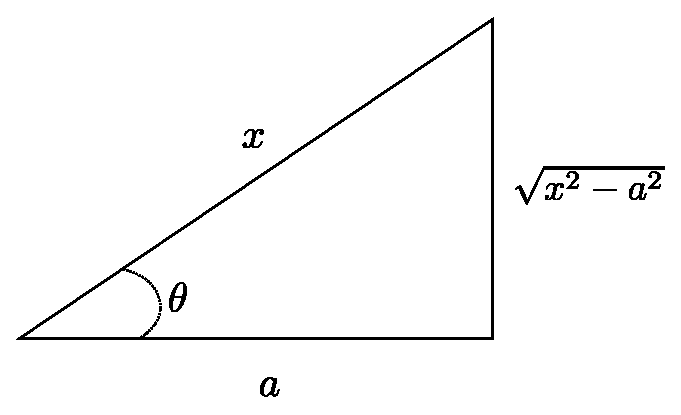
\includegraphics[width=0.4\textwidth]{continuous/integration/asectheta.eps}
  \end{center}
\end{figure}
For integrands with $\sqrt{a^2-x^2}$, let $x=a \sin \theta$ and $\ud x = a \cos \theta \ud \theta$.
\begin{figure}[H]
  \begin{center}
    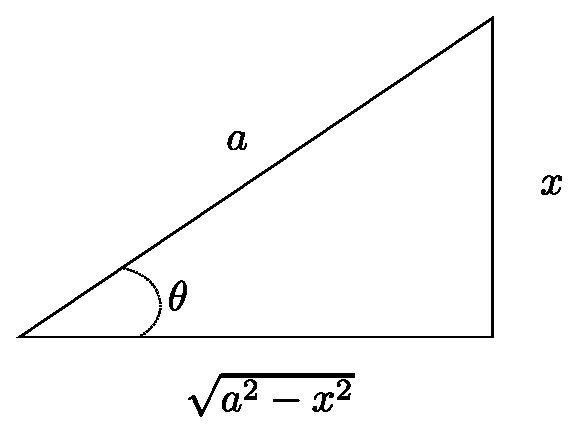
\includegraphics[width=0.4\textwidth]{continuous/integration/asintheta.eps}
  \end{center}
\end{figure}
For integrands with $ \sqrt{x^2+a^2}$, let $x = a \tan \theta$ and $\ud x = \sec^2 \theta \ud \theta$.
\begin{figure}[H]
  \begin{center}
    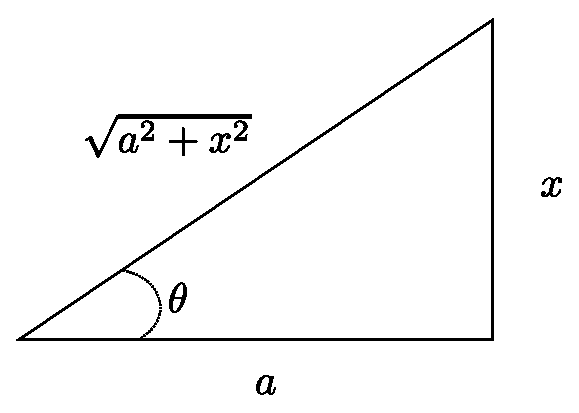
\includegraphics[width=0.4\textwidth]{continuous/integration/atantheta.eps}
  \end{center}
\end{figure}

\begin{ex}
  Integrate
  \[ \int \frac{\ud x}{x \sqrt {x^2 -4}} \]
  \begin{sol}
    Let $x=2 \sec \theta$ and $\ud x = 2 \sec \theta \tan \theta \ud \theta$.
    \begin{align*}
      \int \frac{\ud x}{x \sqrt {x^2 -4}}
      &= \int \frac{2 \sec \theta \tan \theta \ud \theta}{2 \sec \theta \sqrt{4\sec^2 \theta -4}} \\
      &= \int\frac{tan \theta \ud \theta}{\sqrt{4 \sec^2 \theta -4}} \\
      \intertext{Now we use the trigonometric identity $1+\tan^2\theta=\sec^2\theta$.}
      &= \int \frac{\tan\theta\ud\theta}{\sqrt{4(1+\tan^2\theta)-4}}\\
      &= \int \frac{\tan\theta\ud\theta}{\sqrt{4\tan^2\theta}}\\
      &= \int\frac{\tan\theta\ud\theta}{2\tan\theta}\\
      &= \int \frac{1}{2}\ud\theta \\
      &= \frac{1}{2}\theta+C\\
      \intertext{Now we draw a triangle, using the numbers from our original substitution:}
      % add a picture
      &=\frac{1}{2}\arcsec{\frac{x}{2}} +C
    \end{align*}
    \begin{figure}[H]
      \begin{center}
        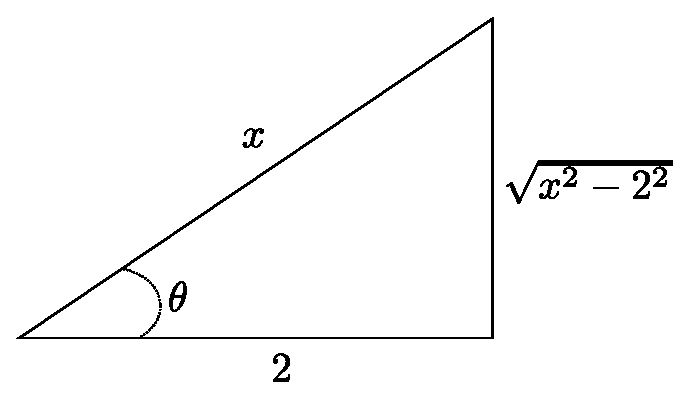
\includegraphics[width=0.4\textwidth]{continuous/integration/secexample.eps}
      \end{center}
    \end{figure}
  \end{sol}
\end{ex}
% \begin{ex}
%   \[ \int \frac{dx} {x \sqrt{x^{2}-4}} \]
%   \begin{sol}
%   \begin{align*}
%     \lets x&=2\sec \theta & \lets dx &= 2 \sec \theta \tan \theta \ud \theta
%   \end{align*}
%   \begin{align*}
% 	  \int \frac{\ud x} {x \sqrt{x^2-4}}
% 	  =&\int \frac{2 \sec \theta \tan \theta \ud \theta}{2 \sec \theta \sqrt{4\sec^2\theta-4}} \\
% 	  =&\int \frac{\tan \theta \ud \theta}{\sqrt{4\sec^2 \theta-4}} \\
% 	  =&\int \frac{\tan \theta}{2 \tan \theta} \ud \theta
% 	  = \frac {1}{2} \theta + C \\
%   \end{align*}
% This is unfinished, we still need to solve for $\theta$.
% \end{sol}
% \end{ex}
\begin{ex}
  \[ \int \frac{\ud x}{\sqrt{1-x^{2}}} = \sin^{-1}x+C \]
\end{ex}
\begin{ex}
  \[ \int \frac{2x}{\sqrt{1-x^2}}dx \]
  \begin{sol}

  \[ \text{let} u = 1-x^{2} \ldots \]
\end{sol}
\end{ex}
\begin{ex}
  \[ \int x^{3} \sqrt {4-x^2} \ud x \]
  \begin{sol} Although perhaps solvable using integration by parts, we will use trigonometric substitution.
  \begin{align*}
    \lets  x &= 2 \sin{\theta} \\ \lets \ud x &= 2\cos \theta \ud \theta
  \end{align*}
  \begin{align*}
    \int x^{3} \sqrt {4-x^2} \ud x
    =&\int 8\sin^3 \theta \, 2\cos\theta \, 2\cos\theta \, \ud\theta
   =32 \int \sin^{3}\theta\cos^{2} \theta \ud\theta \\
   =& 32 \int \sin^{2}\theta\cos^{2} \theta\sin \theta \ud\theta \\
   =& 32 \int (1-\cos^{2}\theta) \cos^{2} \theta\sin \theta \ud\theta \\
   \intertext{Let $u=\cos\theta$ and $\ud u = -\sin \theta \ud \theta$.}
   =&-32 \int (1-u^{2})\,u^{2}\ud u \\
   =&\frac {-32u^3}{3}+\frac{32u^5}{5}+C \\
   =&\frac{-32\cos^{2}\theta}{3}+\frac{32\cos^{5}\theta}{5}+C \\
   =&\frac {-32}{3} \left(\frac{\sqrt{4-x^2}}{2}\right)+\frac {32}{5} \left(\frac{\sqrt{4-x^2}}{2}\right)^5+C \\
 \end{align*}
 \end{sol}
\end{ex}

% \begin{homework}
%   Read Section 8.3.
% \end{homework}

\begin{ex}
  \[ \int \sqrt{x^2+6x} \ud x \]
  \begin{sol}
    \begin{align*}
      \int \sqrt{x^2+6x} \ud x =&\int \sqrt{x^2+6x+9-9}\ud x
      =\int \sqrt{(x+3)^2-9}\ud x \\
      \intertext{Now let $x+3=3\sec\theta$ and $\ud x=3\sec\theta \tan\theta \ud\theta$.}
      =& 3 \int \sqrt{9\sec^2\theta-9}\sec\theta \tan\theta \ud \theta \\
      =& 9 \int \tan^2\theta\sec\theta\ud\theta
  \end{align*}
\end{sol}
\end{ex}
\begin{ex}
  Integrate
    \[ \int \frac{1}{\sqrt{x^2+2x+5}}\ud x \]
  \begin{sol}
    \begin{align*}
      \int \frac{1}{\sqrt{x^2+2x+5}}\ud x
      =& \int \frac{1}{\sqrt{x^2+2x+1+4}} \\
      =& \int \frac{1}{\sqrt{(x+1)^2+4}} \\
      \intertext{Let $u=x+1$ and $\ud u=\ud x$.}
      =& \int \frac{\ud u}{\sqrt{u^2+4}} \\
      =& \arcsin \frac{x+1}{4}+C
    \end{align*}
  \end{sol}
\end{ex}


\section{Partial Fraction Decomposition}
% Unoriginal work. REWRITE THIS!
%
% A rational function $P(x)/Q(x)$ can be rewritten using what is known as partial fraction decomposition. This procedure often allows integration to be performed on each term separately by inspection. For each factor of $Q(x)$ the form $(a\,x+b)^m$:
%
% \begin{equation}
%   \frac{A_1}{a\,x+b}+\frac{A_2}{(a\,x+b)^2}+\ldots+\frac{A_m}{(a\,x+b)^m}
% \end{equation}
%
% For each factor of the form $(a\,x^2+b\,x+c)^m$ introduce terms:
%
% \begin{equation}
%   \frac{A_1\,x+B_1}{a\,x^2+b\,x+c}+\frac{A_2\,x+B_2}{(a\,x^2+b\,x+c)^2}+\ldots+\frac{A_m\,x+B_m}{(a\,x^2+b\,x+c)^m}
% \end{equation}
%
% Then write:
%
% \begin{equation}
%   \frac{P(x)}{Q(x)}=\frac{A_1}{a\,x+b}+\ldots+\frac{A_2\,x+B_2}{(a\,x^2+b\,x+c)^2}+\ldots
% \end{equation}
%
% And solve for $A_i$s and $B_i$s.
%
%
% \subsection{Repeated Linear/Quadratic Den. Factors}
%
% \begin{align*}
%   \frac {\cdots}{\underbrace{(x^2+3)^2}_\text{quadratic} \, \underbrace{(x+1)}_\text{linear} \, \underbrace{(x^2+x+4)}_\text{quadratic}}
%   &=\frac {Ax+B}{(x^2+3)^2} + \frac{Cx+D}{(x^2+3)^1} + \frac {E}{x+1} + \frac {Fx+G}{x^2+x+4}
% \end{align*}
%
% \begin{align*}
%   \frac {\cdots}{(x^2-2x+1)(x^2-4x+4)}
%   &=\frac {\cdots}{(x-1)^2(x-2)^2} \\
%   &=\frac{A}{(x-1)^2}+\frac{B}{x-1}+\frac{C}{(x-2)^2}+\frac{D}{x-2}
% \end{align*}
\subsection{Determining A,B,C, \dots}

% This is just BAD. Really bad. Jesus, fix this.

Multiply the denominator by both sides of the new equation:
\[ {denominator}*\left[\frac{x^3+2x^2+x+8}{(x^2+4)^2}\right]=\left[\frac{Ax+B}{(x^2+4)^2}+\frac{Cx+D}{(x^2+4)^1}\right]*{denominator} \]

Now solve for \(A\), \(B\), and \(C\).

\begin{align*}
  x^3+2x^2+x+8 &= (Ax+B)+\,(Cx+D)(x^2+4)\\
  x^3+2x^2+x+8 &= (Ax+B)+Cx^3+4Cx+Dx^2+4D
\end{align*}

Now:
\begin{table}[H]
  \centering
  \begin{tabular}{r|l}
    \(x^2\) terms & \( 2=D \) \\
    \(x\) terms & \( 1 = A + 4C  \) \\
    const terms & \( 8 = B + 4D \)
  \end{tabular}
\end{table}

\subsection{Factoring}

\begin{equation}
  (F)^3+(L)^3=(F+L)(F^2-FL+L^2)
\end{equation}
\begin{equation}
  (F)^3-(L)^3=(F-L)(F^2+FL+L^2)
\end{equation}
Note: you cannot factor a sum of perfect squares.
\begin{remark} When factoring quadratics, consider the discriminant (from the quadratic formula at \ref{app:eq:quadratic}):
  \begin{align*}
    &10x^2-x-2 \\
    &b^2-4ac \\
    &(-1)^2-4(10)(-2)
  \end{align*}
\end{remark}

% \begin{homework} From \emph{Thomas' Calculus}, solve
%
%   \begin{tabular}{llr}
%     page & problems & sols \\ \hline
%     475 & 25 \\ & 27 (b) \\ & 32 \\
%     492 & 70 & $\frac{-x^2}{2}-\frac{3}{2}\ln{|x+2|}-\frac{5}{2}ln{|x-2|}$ \\
%     & 72 & ($\sin^1{x+1}$) \\
%     & 75 \\
%     & 75 & $\frac{x^2}{2}+2x+3ln{|x-1|}-\frac{1}{x-1}$ \\
%     & 79 \\ &83\\&85\\&86&$\frac{x^2-1}{2}e^{x^2}$\\&87\\&88&$\frac{-\tan^{-1}x}{x}+\ln{|x|}-\ln{\sqrt{|1+x^2}|}$\\&99\\&101\\
%   \end{tabular}
% \end{homework}


% \section{Test Review}
% \begin{comment}
% \begin{ex}
%   $$ \int cot^3 (2x)\ud x $$
%   $$ \int (csc^2 2x -1) \, cot2x \ud x $$
%   $$ \int csc^2 2x\, cot \, 2x \ud x - \int \frac {cos\,2x}{sin\,2x}\ud x $$
%   $$ \text {abandoned ...} $$
% \end{ex}
% \end{comment}
% %\begin{ex}
% %  Integrate \[ \int \sqrt{16-9x^2} \ud x \]
% %  \begin{sol}
% %  Factor out a $9$.
% %  \begin{align*}
% %    \int \sqrt{16-9x^2} \ud x
% %    =& \int \sqrt{9\left(\frac{16}{9}-x^2\right)} \ud x
% %    =3 \int \sqrt{\frac{16}{9}-x^2} \ud x \\
% %    \intertext{Let $x= \frac{4}{3}\sin \theta$ and $\ud x = \frac{4}{3}\cos \theta \ud \theta$.}
% %    =& 3 \int \sqrt{\frac{16}{9}-\left( \frac{4}{3}\sin\theta \right)^2}\,\frac{4}{3}\cos\theta\ud\theta \\
% %    =& 3 \int \sqrt{\frac{16}{9}-\frac{16}{9}\sin^2\theta}\,\frac{4}{3}\cos\theta\ud\theta \\
% %    =& 3 \int \frac{4}{3}\sqrt{1-\sin^2 \theta} \,\frac{4}{3}\cos\theta\ud\theta \\
% %    =& \frac{16}{3} \int \sqrt{\cos^2\theta}\cos\theta\ud\theta \\
% %    =& \frac{16}{3} \int \cos^2\theta\ud\theta
% %  \end{align*}
% %  \center{[Incomplete. See comments for details.]}
% %\end{sol}
% %\end{ex}
% %\begin{ex}
% %  $$ \int \sqrt{16-9x^2} \ud x $$
% %  $$ \int \sqrt{9\frac{16}{9}-x^2}\ud x $$
% %  $$ \text {try } x = \frac{4}{3}\sin \, \theta $$
% %  $$ dx = \frac{4}{3}cos\,\theta \, \ud \theta $$
% %  $$ 3 \int \sqrt{\frac{16}{9}-x^2}\ud x $$
% %  $$ 3 \int \sqrt{\frac{16}{9}-\frac{16}{9}sin^2 \, \theta } \, \frac{4}{3}cos\,\theta \, d\theta $$
% %  $$ 3 \int \frac {4}{3} \sqrt{cos^2 \, \theta } \frac{4}{3} cos\,\theta\,d\theta $$
% %  $$ \frac{16}{3} \int cos^2 \theta \, d \theta $$
% %  $$ \frac{16}{3}\left[\frac{\theta}{2}+\frac{sin\,2\theta}{4}\right] $$
% %  $$ \theta = sin^{-1}\,\frac{3x}{4} $$
% %  $$ \frac{16}{3}\left[\frac{sin^{-1}\,\frac{3x}{4}}{2}+\frac{sin\,2(sin^{-1}\,\frac{3x}{4})}{4}\right] $$
% %\end{ex}

\subsection{Examples}

\begin{ex}
  \begin{align*}
    \frac{x+3}{x^2-3x+2}
   =&\frac{x+3}{(x-2)(x-1)} \\
   =&\frac{A}{x-2}+\frac {B}{x-1}
  \end{align*}
\end{ex}
\begin{ex}
  \begin{align*}
    \frac {x+3} {x^4+3x^3+6x^2+12x+8}
    =&\frac {x+3} {(x^2+4)(x+1)(x+2)} \\
    =&\frac{A}{x+1}+\frac{b}{x+2}+\frac{Cx+D}{x^2+4}
  \end{align*}
\end{ex}
\begin{ex}
  \begin{align*}
    \frac{x+3}{x^4+5x^2+4}
    =&\frac{x+3}{(x^2+4)(x^2+1)}\\
    =&\frac{Ax+B}{x^2+4}+\frac{Cx+D}{x^2+1}
  \end{align*}
\end{ex}
\begin{ex}
  \begin{align*}
    \frac{1}{x^2-1}
    =&\frac{1}{(x-1)(x-1)} \\
    =&\frac{A}{x+1}+\frac{B}{x-1}
  \end{align*}
\end{ex}
\begin{ex}
  \begin{align*}
    \frac{1}{x^2-x}
     =&\frac{1}{x(x-1)} \\
     =&\frac{A}{x}+\frac{B}{x-1}
  \end{align*}
\end{ex}

\begin{ex}
  \begin{align*}
   \frac {9x^2+7x-4}{x^3-3x^2-4x} \\
   \frac {9x^2+7x-4}{x(x^2-3x-4)} \\
   \frac {9x^2+7x-4}{x(x-4)(x+1)} \\
   \frac{A}{x}+\frac{B}{x-4}+\frac{C}{x+1}
  \end{align*}
\end{ex}
\begin{ex}
  \begin{align*}
   \frac {x+3}{x^2-4} \neq \frac {A}{x+2} + \frac {B}{x-2} \\
   \frac {x+3}{x^2-4} = \frac {x^3+0x^2+0x+4}{x^2-4} \\
   \frac {x+3}{x^2-4} = x + \underbrace{\frac {4x+4}{x^2-4}}_{\frac{A}{x+2}+\frac{B}{x-2}}
 \end{align*}
\end{ex}
\begin{ex}
  \[ \int \frac{8x^4+6x^2-3x+1}{2x^2-x+2} \]
  \begin{sol}
  Use long division to simplify as follows:
    \begin{center}
      \polylongdiv{8x^4+6x^2-3x+1}{2x^2-x+2}
    \end{center}
    \begin{align*}
      \frac{8x^4+6x^2-3x+1}{2x^2-x+2} &=
      4x^2+2x+\frac{\overbrace{-7x+1}^{Ax+B}}{2x^2-x+2}
    \end{align*}
    So
    \begin{align*}
      \int \frac{8x^4+6x^2-3x+1}{2x^2-x+2}
      &= \int 4x^2+2x+\frac{-7x+1}{2x^2-x+2}
    \end{align*}
    Then solve.
  \end{sol}
\end{ex}
\begin{ex}
  \[ \int \frac{dx}{x^2+2x} \]
  \begin{sol}
    Note that
    \[ \left[ \frac{1}{x^2+2x}\right] \text{ is }
    \left[\frac{A}{x}+\frac{B}{x+2}\right] \]
    \begin{align*}
      \int \frac{\ud x}{x^2+2x} &=
      \int \frac{\frac{1}{2}}{x}+\frac{\frac{1}{2}}{x+2} \ud x \\
      &= \int \frac{\frac{1}{2}}{x} \ud x+\int\frac{\frac{1}{2}}{x+2} \ud x \\
      &= \frac{1}{2}\ln{|x|}+\frac{-1}{2}\int\frac{\ud u}{u} \\
      &= \frac{1}{2}\ln{|x|}+\ln{|x+2|}
    \end{align*}
  \end{sol}
\end{ex}

\begin{ex}
  Write the partial fraction decomposition of
  \[ \frac{1}{x^4+2x^2+1} \]
  \begin{sol}
    It's a trinomial, so we know we have to try binomial times binomial--and that works.
    \begin{align*}
	    \frac{1}{x^4+2x^2+1}
	      &=\frac{1}{(x^2+1)(x^2+1)}
	       =\frac{Ax+B}{(x^2+1)^2}+\frac{Cx+D}{x^2+1}
	    \intertext{Multiply both sides by the denominator}
	      &=Ax+B+(x^2+1)(Cx+D)
    \end{align*}
    Now, solve for A, B, C, and D.
    \begin{align*}
      1&=Ax+B+(x^2+1)(Cx+D) \\
      1&=B+D \\
      0&=A+C \\
      0&=C \\
      0&=D
    \end{align*}
    So A is 0, B is 1, C is 0, and D is 0.
  \end{sol}
\end{ex}
%\subsection{Integrals}
%$$\int \frac{dx}{x^2-16} $$
%$$ (x^2-16)*\left[\frac{1}{(x+4)(x-4)}\right=\left[\frac{A}{(x+4)}+\frac{B}{x-4}\right]*(x^2-16) $$
%$$ 1 = A(x-4)+B(x+4) $$
\begin{ex}
  Integrate
  \[ \int \frac{1}{(x+1)(x-1)} \]

  \begin{sol}
  \begin{align*}
    \int \frac{1}{(x+1)(x-1)}
      =& \int \frac{A}{x+1}+\frac{B}{x-1}\ud x \\
    \intertext{Solve for $A$ and $B$.}
      =& \int \frac{-1/2}{x+1}+\frac{1/2}{x-1} \\
      =& \frac{-1}{2} \int \frac{\ud x}{x+1}
         + \frac{1}{2} \int \frac{\ud x}{x-1}
  \end{align*}
\end{sol}
\end{ex}
\begin{ex}
  Integrate
  \[ \int \frac{x^2}{x+8} \ud x \]
  \begin{sol}
    Use long division to simplify the integrand:
    \begin{center}
      \polylongdiv{x^2+0x+0}{x+8}
    \end{center}
      \begin{align*}
        \int \frac{x^2}{x+8} \ud x
        =&\int x-8 + \frac{64}{x-8}\ud x\\
        =&\frac{1}{2}x^2-8x+64\ln{|x+8|}+C
      \end{align*}
  \end{sol}
\end{ex}
\begin{ex}
  Integrate
  \[ \int \frac{1}{x^2-5x-6}\ud x \]
  \begin{sol}
    Use partial fraction decomposition:
    \begin{align*}
    \frac{1}{x^2-5x-6} = \frac{1}{(x-6)(x+1)}\\
    \frac{1}{(x-6)(x+1)} = \frac{A}{x-6}+\frac{B}{x+1} \\
    1 = A(x+1)+B(x-6) \\
    1 = Ax+A+Bx-6B \\
    1 = Ax+Bx+A-6B \\
    \end{align*}
    If $x=0$, then $A-6B=1$. If $x=1$, then $2A-5B=1$. We can substitute the first equation into the second to get
    \begin{align*}
      2(1+6B)-5B&=1 \\
      2+12B-5B&=1 \\
      B&=-1/7 \\
    \end{align*}
    \begin{align*}
      A-6B&=1 \\
      A-6(1/7)&=1 \\
      A&=1/7 \\
    \end{align*}
    \begin{align*}
      \frac{1}{x^2-5x-6}=&\frac{1/7}{x-6}-\frac{1/7}{x+1} \\
      \int \frac{1}{x^2-5x-6}\ud x=&\int  \frac {1/7}{x-6}-\frac{1/7}{x+1} \ud x \\
      =& \frac{1}{7} \int \frac{1}{x-6}-\frac{1}{x+1}\ud x \\
      =& \frac{1}{7}\left(\ln{|x-6|}-\ln{|x+1|}\right)+C
    \end{align*}
  \end{sol}
\end{ex}
\section{Simpson's Rule}
\begin{ex}
  Estimate
  \[ \int^5_1 \frac{1}{x}\ud x \]
  using the trapezoidal rule with four trapezoids.
  \begin{remark}
    For one trapezoid:
      \[ \frac{\Delta x}{2}(y_0+y_1) \]
    For the entire Trapezoid Rule:
      \[ \frac{\Delta x}{2}(y_0+2y_1+2y_2+2y_3+\dots+y_n) \]
    For full-blown Simpson's Rule:
      \[ \frac{\Delta x}{3}(y_0+4y_1+2y_2+4y_3+ \dots +2y_{n-2}+ 4y_{n-1}+y_n) \]
  \end{remark}
  \begin{remark}
    The question might be seen as: ``\dots using the trapezoidal rule with $n=4$.''
  \end{remark}
  \begin{sol}
  \begin{align*}
    \int^5_1 \frac{1}{x}\ud x
      \approx & \frac{\overbrace{\Delta x}^1}{2}
        \left(\frac{1}{1}+2 \frac{1}{2}+2 \frac{1}{3}+ 2 \frac{1}{4}+1 \frac{1}{5}\right)
        \\
      =& \frac{1}{2}(2^{1/2}+2/3+1/5) \\
      =& \frac{1}{2}(5/2+13/15) \\
      =& \frac{101}{60}
  \end{align*}
\end{sol}
\end{ex}
\begin{ex}
  Estimate
  \[ \int^5_1 \frac{1}{x}\ud x \]
  using Simpson's Rule with $n=8$.

  \begin{sol}
  \begin{align*}
  \int^5_1 \frac{1}{x}\ud x
   \approx & \frac{\overbrace{\Delta x}^{1/2}}{3}
     \left(\frac{1}{1}+4 \frac{1}{3/2}+2 \frac{1}{2} + 4 \frac{1}{5/2}+ \dots \right)
  \end{align*}
  Not a real problem, so not finished.
\end{sol}
\end{ex}


\section{Improper Integrals}

\begin{defn}
\emph{Improper integrals} occur in cases where you are integrating across an infinite domain or infinite range.
\end{defn}

\begin{figure}[H]
  \begin{center}
    \begin{tikzpicture}
      \begin{axis}[
        ylabel={$\frac{1}{\sqrt{x}}$},
        axis x line=bottom,
        axis y line=center,
        tick align=outside,
        axis y discontinuity=crunch,
        xtickmax=10,
        ytickmin=10,
        ]
        \addplot {1/sqrt(x)};
      \end{axis}
    \end{tikzpicture}
  \end{center}
  \caption{An example of a function that can produce improper integrals.}
\end{figure}


\subsection{Infinite Range}

\begin{ex}
	\[ \int^{9}_1 \frac{1}{x-4}\ud x \]
	Right and left approach problem spot.
\end{ex}
\begin{ex}
	\[ \int^{39}_{4}\frac{1}{\sqrt{x-4}}\ud x \]
	Right approach problem spot.
\end{ex}
\begin{ex}
	\[ \int^0_{-4} \ln{|x|} \ud x \]
	Left approach problem spot.
\end{ex}
\begin{ex}
  \[ \int^{10 \pi}_{-6\pi} \sec x \ud x \]
  Problems with right and left approach.
\end{ex}
\begin{ex}
This is considered a ``Classic.''
  \begin{align*}
    &\int^{b}_{a} \frac{1}{(b-x)^p} \ud x && \text{and} &&\int^{b}_{a} \frac{1}{(x-a)^p} \ud x
  \end{align*}
\end{ex}
\begin{ex}
  Integrate:
    \[ \int^{-2}_{-6} \frac{1}{(x+6)^1} \ud x \]
  \begin{sol}
    \begin{align*}
      \int^{-2}_t \frac{1}{x+6} \ud x
      =& \ln{|x+6|}\bigg|^{-2}_t \\
      =& \lim_{t \to -6^+} \ln{|-2+6|}-\underbrace{\ln{|-6^++6|}}_\text{Diverges.}
    \end{align*}
  \end{sol}
\end{ex}
\begin{ex}
  Integrate:
    \[ \int^{6}_{2} \frac{1}{(x-6)^2} \ud x \]
  \begin{sol}
  \begin{align*}
    \int^{t}_2 \frac{1}{x+6} \ud x
    =& \frac{(x-6)^{-1}}{-1} \bigg|^t_2 \\
    =& \lim{t \to 6^-} \frac{(t-6)^{-1}}{-1}-\frac{(2-6)^{-1}}{-1}
  \end{align*}
\end{sol}
\end{ex}
\begin{ex}
  Integrate:
  \begin{align*}
    \int^{3}_{1} \frac{1}{\sqrt{x-1}}
    =& \frac{(x-1)^{1/2}}{1/2}\bigg|^3_t \\
    =& \lim_{t \to 1+} \frac{(3-1)^{1/2}}{1/2}-\frac{(t-1)^{1/2}}{1/2}
  \end{align*}
\end{ex}
\begin{ex}
  Integrate.
  \[ \int^{39}_4 \frac{1}{\sqrt{x-4}} \ud x \]
  Substitute with $4 \to t$:
  \[ \int^{39}_t \frac{1}{\sqrt{x-4}} \ud x \]
  And evaluate:
  \begin{align*}
    \int^{39}_t \frac{1}{\sqrt{x-4}} \ud x
    =& \lim_{t \to 4^+} \frac{(x-4)^{1/2}}{1/2} \bigg|^{39}_t \\
    =& \lim_{t \to 4^+} \frac{(39-4)^{1/2}}{1/2}-\frac{(t-4)^{1/2}}{1/2} \\
    =& \frac{(39-4)^{1/2}}{1/2}
  \end{align*}
\end{ex}
\begin{ex}
  Integrate.
  \[ \int^{29}_1 \frac{1}{x-4} \ud x \]
  \begin{sol}
    Substitute $29 \to t$:
    \begin{align*}
      \int^{29}_1 \frac{1}{x-4} \ud x =& \int^t_1 \frac{1}{x-4} \ud x
      + \int^{29}_t \frac{1}{x-4} \ud x \\
      &= \ln{|x-4|}\bigg|^t_1 + \ln{|x-4|} \bigg|^{29}_t \\
      &=\ln{|t-4|}-\ln{|1-4|}+\ln{|29-4|}-\ln{|t-4|} \\
      &=\lim_{t \to 4^-} \left[\underbrace{\ln{|t-4|}}_{\frac{1}{-\infty}}-\ln{|1-4|}\right]+\lim_{t \to 4^+} \left[\ln{|29-4|}-\underbrace{\ln{|t-4|}}_{\frac{1}{\infty}}\right]
    \end{align*}
    Diverges.
  \end{sol}
\end{ex}
\begin{ex}
  Integrate:
  \[ \int^5_0 \ln{x} \ud x \]
  \begin{sol}
  \begin{align*}
    \int^5_t \ln{x} \ud x =&x \ln{x} -x \bigg|^5_t \\
    &=5 \ln{5} -5-t\ln{t}+t \\
    \intertext{Now evaluate the limit as:}
    \int^5_0 \ln{x} \ud x =& \lim_{t \to 0^+}5 \ln{5} -5-t\ln{t}+t \\
    &=5 \ln 5 - 5
  \end{align*}
\end{sol}
\end{ex}

% \begin{homework}
%   4th online homework assignment due SUNDAY at end of break.
%
%   Read section 8.7.
%
%   pg. 487 \#3, 4 (4), 5, 6, ($\frac{-9}{2}$), 7, 8 (1000), 15, 25, 26 (1)
% \end{homework}

\subsection{Infinite Domain}

For these, the integrand is well behaved throughout the integration interval. The problem is that we are integrating across an interval $[a, b]$ where either $a$ or $b$ is $\infty$ or $-\infty$.

\begin{equation}
  \int^{\infty}_{\#} f(x) \ud x
\end{equation}
We would treat this an indefinite integral:
\[ \int f(x) \ud x = F(x) \]
Then evaluate it as follows:
\[ \lim_{t \to \infty} F(x)\bigg|^{t}_{\#} \] \\

\begin{equation}
  \int^{\#}_{-\infty} f(x) \ud x
\end{equation}
Like the first one, we would treat this as an indefinite integral:
\[ \int f(x) \ud x = F(x) \]
Then evaluate it as follows:
\[ \lim_{t \to \infty} F(x)\bigg|^{\#}_{-\infty} \] \\

Others, still, look like this:
\begin{equation}
  \int^{\infty}_{-\infty} f(x) \ud x
\end{equation}
Treat this as a combination of two of the above integrals. Rewrite it as:
\[ \int^{a}_{-\infty} f(x) \ud x
    + \int^{\infty}_{a} f(x) \ud x \]
choosing some arbitrary \(a\), which we usually choose to be \(0\).

\begin{ex}
    For $p>1$, does the following integral converge or diverge?
    \[ \int^\infty_1 \frac{1}{x^p} \ud x \]
    \begin{sol}
      The integral converges.
    \end{sol}
  \end{ex}
\begin{ex}
	\[ \int^{\infty}_1 x^{-3} \ud x \]
	\begin{sol}
	\begin{align*}
		\int^{\infty}_1 x^{-3} \ud x &=\lim_{t \to \infty} \frac{x^{-2}}{2}\bigg|^{t}_{1} \\
		  &=\lim_{t \to \infty} \frac{t^{-2}}{-2}-\frac{1^{-2}}{-2} \\
		  &=\lim_{t \to \infty} \frac{1}{-2t^2}+\frac{1}{2}
	\end{align*}
The integral converges to $1/2$.
\end{sol}
\end{ex}
\begin{ex}
	\[ \int^\infty_1 \frac{1}{\sqrt{x}}\ud x \]
	\begin{sol}
	\begin{align*}
		\int^\infty_1 \frac{1}{\sqrt{x}}\ud x &=\lim_{t \to \infty} \frac{x^{1/2}}{\frac{1}{2}}\bigg|^t_1 \\
		&=\lim_{t \to \infty} \frac{t^{1/2}}{\frac{1}{2}}-\frac{1^{1/2}}{\frac{1}{2}} \\
		&=\lim_{t \to \infty} 2t^{1/2}-2
	\end{align*}
The integral diverges.
\end{sol}
\end{ex}
\begin{ex}
	\[ \int^\infty_0 \frac{1}{x^2+1} \]
	\begin{sol}
	\begin{align*}
		\int^\infty_0 \frac{1}{x^2+1} &= \lim_{t \to \infty} \arctan x \bigg|^t_0 = \lim_{t \to \infty} \arctan t - \arctan 0 \\
		&= \lim_{t \to \infty} \arctan t \\
		&= \lim_{t \to \infty} \arctan t \\
		&= \frac{\pi}{2}
	\end{align*}
  \begin{figure}[H]
    \begin{center}
        \subfigure[\(f(x)=\tan{x}\).]{
          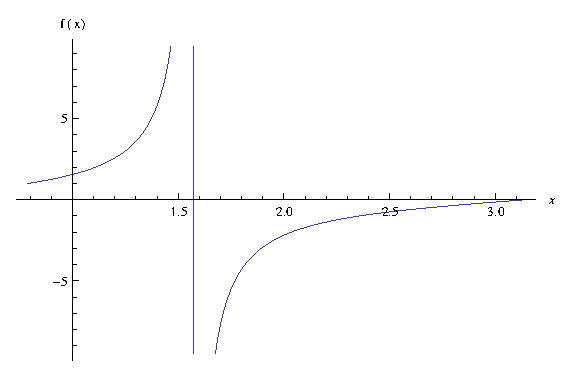
\includegraphics[scale=0.8]{graphs/tanx.eps}
        }
        \subfigure[\(f(x)=\arctan{x}\).]{
          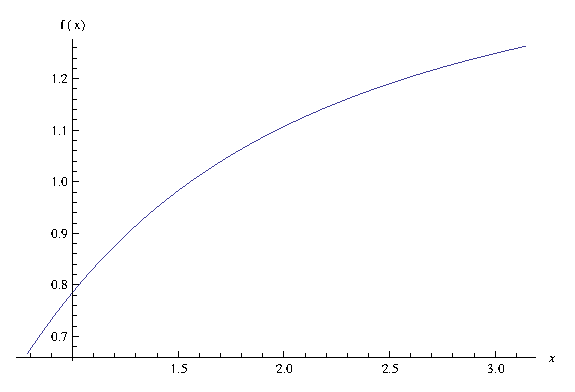
\includegraphics[scale=0.8]{graphs/arctanx.eps}
        }
    \end{center}
    \caption{\(\tan x\) compared with \(\arctan x\).}
  \end{figure}
  \end{sol}
\end{ex}
\begin{ex}
	\[ \int^0_{-\infty} \frac{x^2}{x^3-1} \]
	\begin{remark}
	  If $0 \to 1$, this would be a Type I integral.
	\end{remark}
	\begin{sol}
	  \begin{align*}
	  	\int^0_{-\infty} \frac{x^2}{x^3-1} &=\int^0_{-\infty} \frac{1}{3} \frac{\ud u}{u} \\
	  	&= \lim_{t \to \infty} \frac{1}{3}\ln{|x^3-1|\bigg|^0_t}
	  	= \lim_{t \to \infty} \frac{1}{3} \ln{|-1|}-\frac{1}{3}\ln{|t^3-1|} \\
	  	&= \lim_{t \to \infty} \frac{1}{3}ln{1}-\frac{1}{3}\ln{|t^3-1|} \\
	  	&= \lim_{t \to \infty} -\frac{1}{3}\ln{|t^3-1|}
	  \end{align*}
    The integral diverges.
  \end{sol}
\end{ex}
\begin{ex}
	\[ \int^0_{-\infty} e^x \ud u \]
	\begin{remark}
	  This is likely to converge, because of the $e^{-\infty}$.
	\end{remark}
	\begin{sol}
	\begin{align*}
		\int^0_{-\infty} e^x \ud u & =\lim_{t \to -\infty} e^x \bigg|^0_t \\
		&=\lim_{t \to -\infty} e^0-e^t
	\end{align*}
	The integral converges to $1$.
  \end{sol}
\end{ex}
\begin{ex}
	\[ \int^\infty_{-\infty} e^{-x} \cos x \ud x \]
	\begin{sol}
  First, break this into two parts.
	\begin{align*}
		\int^\infty_{-\infty} e^{-x} \cos x \ud x
		&=\int^0_{-\infty} e^{-x} \cos x \ud x+\int^\infty_0 e^{-x} \cos x \ud x \\
		\intertext{Then, treat it as an indefinite integral and evaluate using integration by parts:}
		\int e^{-x} \cos x \ud x&=\frac{e^{-x}\sin x - e^{-x} \cos x}{2}
		\intertext{Now, return to our original function.}
		\lim_{t \to \infty} e^{-x} \cos x \ud x
		&=\lim_{t \to \infty}
		  \frac{e^{-x}\sin x - e^{-x} \cos x}{2}\bigg|^0_t
		  -\frac{e^{-x}\sin x - e^{-x} \cos x}{2}\bigg|^t_0 \\
		&=\lim_{t \to \infty}
		  \left[\frac{e^{-0}\sin  - e^{-0} \cos 0}{2}
		  -\frac{e^{-t}\sin t - e^{-t} \cos t}{2}\right]
		  -\left[0+\frac{1}{2}\right] \\
	\end{align*}
	Because the left half of this diverges, the entire integral diverges.
\end{sol}
\end{ex}
\begin{ex}
  This is one of the classics:
	\[ \int^\infty_1 \frac{1}{x}\ud x \]
	\begin{sol}
	  Consider:
    \[ \int^\infty_1 \frac{1}{x^{1.000000001}}\ud x = x^{-0.000000001}\bigg|^\infty_1=0-\frac{1}{1^{0.000000001}}\]
    Therefore:
	  \begin{align*}
	  	\int^\infty_1 \frac{1}{x}\ud x
	  	&=\lim_{t \to \infty} \ln{|x|}\bigg|^t_1=\lim_{t \to \infty} \ln{|t|}-\ln{|1|} \\
	  	& =\lim_{t \to \infty} \ln{|t|}
	  \end{align*}
	  Diverges.
  \end{sol}
\end{ex}
\begin{ex}
  \[ \int^\infty_1 \frac{1}{x^2}\ud x =\lim_{t\to\infty}
    \frac{x^{-1}}{-1}\bigg|^t_1 \]
  This integral converges.
\end{ex}

\section{Test Review}
\begin{ex}
  \[ \int \tan x \sec^4x \ud x \]
  \begin{sol}
    Set aside a $\sec^2x$
    \begin{align*}
      \int \tan x\sec^4x \ud x
      = \int \tan x \sec^2 x \sec^2 x \ud x
    \end{align*}
    Remembering our basic trig identity
    \[ \sin^2x + \cos^2x = 1\]
    we can divide through by $\cos^2x$ to get
    \[ \tan^2x+1=\sec^2x \]
    and substitute that into our new integral
    \begin{align*}
      \int \tan x \sec^2 x \sec^2 x \ud x
      =& \int \tan x (\tan^2x-1) \sec^2x \ud x \\
    \end{align*}
    Now let $u=\tan x$ and $\ud u = \sec^2x \ud x$
    \begin{align*}
      \int \tan x (\tan^2x-1) \sec^2x \ud x
      =& \int u (u^2-1) \ud u \\
      =& \frac{u^3}{3}-\frac{u^2}{2}+C \\
      =& \frac{\tan^3x}{3}-\frac{\tan^2x}{2} +C
    \end{align*}
  \end{sol}
\end{ex}
\begin{ex}
  \[ \int x^2 e^x \ud x \]
  \begin{sol}
    \begin{align*}
      \int x^2 e^x\ud x
      =& x^2 e^x-2\int x e^x \ud x \\
      =& x^2 e^x -2 \left( x e^x - \int e^x \ud x \right) \\
      =& x^2 e^x -2 x e^x +2x +C
    \end{align*}
  \end{sol}
\end{ex}
\begin{ex}
  \[ \int^4_2 \frac{1}{x-4}\ud x \]
  \begin{sol}
    \begin{align*}
      \int^4_2 \frac{1}{x-4}\ud x
      =& x\ln{|x-4|}\bigg|^t_2 \\
      =& \ln{|t-4|}-\ln{|-2|}
    \end{align*}
    Now we go back to the original integral
    \[
      \int^4_2 \frac{1}{x-4}\ud x
      = \lim_{t \to 4^-}\ln{|t-4|}-\ln 2
      \]
      Remembering the graph of \(\ln{|x|}\)
      \begin{figure}[H]
        \begin{center}
          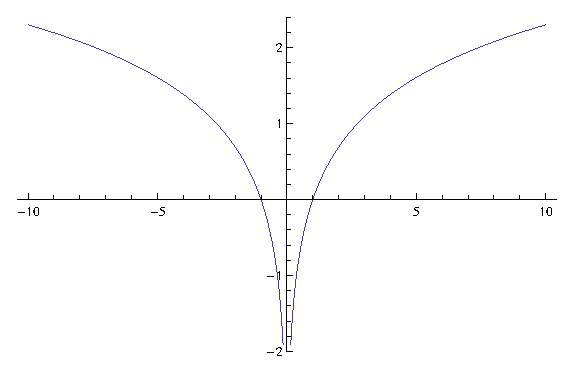
\includegraphics[scale=1]{graphs/logabsx.eps}
        \end{center}
        \caption{A plot of \(f(x)=\ln{|x|}\)}
      \end{figure}
      we can conclude that the integral diverges toward $-\infty$.
  \end{sol}
\end{ex}
\begin{ex}
  \[ \int^6_5 \frac{1}{(x-5)^{1/2}}\ud x \]
  \begin{sol}
    \begin{align*}
      \int^6_t \frac{1}{(x-5)^{1/2}}\ud x
      =& 2 \sqrt{x-5}\bigg|^6_t \\
      =& 2 \sqrt{6-5}-2\sqrt{t-5}
    \end{align*}
    \begin{align*}
      \int^6_5 \frac{1}{(x-5)^{1/2}}\ud x
      =& \lim_{t \to 5^+} 2\sqrt{6-5}-\underbrace{2\sqrt{t-5}}_{0} \\
      =& \lim_{t \to 5^+} 2\sqrt{6-5}\\
      =& 2
    \end{align*}
  \end{sol}
\end{ex}
\begin{ex}
  \[ \int^\infty_{\frac{8\sqrt 3}{3}}\frac{1}{x^2+64}\ud x \]
  \begin{sol}
    \begin{align*}
      \int \frac{1}{x^2-64}\ud x
      =& \int \frac{1}{64(\frac{x^2}{64}+1)} \\
      =&\frac{1}{8}\arctan{\frac{x}{8}} + C
    \end{align*}
    \begin{align*}
      \int^t_{\frac{8\sqrt 3}{3}}\frac{1}{x^2+64}\ud x
      =&\frac{1}{8}\arctan{\frac{x}{8}}\bigg|^t_{\frac{8\sqrt 3}{3}} \\
    \end{align*}
    \begin{align*}
      \int^\infty_{\frac{8\sqrt 3}{3}}\frac{1}{x^2+64}\ud x
      =& \lim_{t \to \infty} \frac{1}{8}\arctan{\frac{t}{8}}-\frac{1}{8}\arctan{\frac{\sqrt 3}{3}} \\
      =& \frac{1}{8}\left(\frac{\pi}{2}-\frac{\pi}{6}\right) \\
      =& \frac{\pi}{24}
    \end{align*}
  \end{sol}
\end{ex}
\begin{ex}
  \[\int x^3 \cos{3x} \ud x\]
  \begin{sol}
    We use integration by parts.
    \begin{align*}
      \int x^3 \cos{3x} \ud x
      =& \frac{1}{3}x^3\sin{3x}-\int x^2 \sin{3x}\ud x \\
      =& \frac{1}{3}x^3\sin{3x}-\left[
        \frac{-1}{3}x^2\cos{3x}+\frac{2}{3}\int x \cos{3x} \ud x
        \right] \\
        =& \frac{1}{3}x^3\sin{3x}+\frac{1}{3}x^2\cos{3x}-\frac{2}{3}\left[\frac{1}{3}x\sin{3x}-\frac{1}{3}\int \sin{3x}\ud x\right] \\
        =&\frac{1}{3}x^3\sin{3x}+\frac{1}{3}x^2\cos{3x}-\frac{2}{9}x\sin{3x}-\frac{2}{27}\cos{3x}+C
    \end{align*}
  \end{sol} \end{ex}

% \begin{homework}
%   Chapter 8 test on Friday, March 16, 2012.
% \end{homework}


